% arara: xelatex
% arara: xelatex
% arara: xelatex


% options:
% thesis=M master's thesis
% english thesis in English language
% hidelinks remove colour boxes around hyperlinks
\documentclass[thesis=M,english,hidelinks]{FITthesis}[2012/10/20]

\usepackage[utf8]{inputenc} % LaTeX source encoded as UTF-8
% \usepackage[latin2]{inputenc} % LaTeX source encoded as ISO-8859-2
% \usepackage[cp1250]{inputenc} % LaTeX source encoded as Windows-1250

\usepackage{graphicx} %graphics files inclusion
% \usepackage{subfig} %subfigures
% \usepackage{amsmath} %advanced maths
% \usepackage{amssymb} %additional math symbols

\usepackage{dirtree} %directory tree visualisation

\usepackage{xcolor} %color
\usepackage{colortbl}
\usepackage{array}

\usepackage{longtable}
\usepackage{booktabs}
\usepackage{tikz}

\usepackage{listings}
\usetikzlibrary{automata,positioning}
\definecolor{Gray}{gray}{0.85}

\newcolumntype{a}{>{\columncolor{Gray}}m}
\newcolumntype{b}{>{\columncolor{white}}m}

\newcommand{\sur}[1]{\ensuremath{^{\textrm{#1}}}}
\newcommand{\sous}[1]{\ensuremath{_{\textrm{#1}}}}

% list of acronyms
\usepackage[acronym,nonumberlist,toc,numberedsection=autolabel]{glossaries}
\newacronym{wep}{WEP}{Wired Equivalent Privacy}
\newacronym{wpa}{WPA}{Wi-Fi Protected Access}
\newacronym{wpa2}{WPA2}{Wi-Fi Protected Access 2}
\newacronym{krack}{KRACK}{Key Reinstallation Attack}
\newacronym{ap}{AP}{Access Point}
\newacronym{lan}{LAN}{Local Area Network}
\newacronym{wlan}{WLAN}{Wireless Local Area Network}
\newacronym{phy}{PHY}{physical layer}
\newacronym{vpn}{VPN}{Virtual Private Networking}
\newacronym{ieee}{IEEE}{Institute of Electrical and Electronics Engineers}
\newacronym{mac}{MAC}{Media access control}
\newacronym{iso}{ISO}{International Standards Organization}
\newacronym{man}{MAN}{Metropolitan Area Network}
\newacronym{lmsc}{LMSC}{LAN/MAN Standards Committee}
\newacronym{wg}{WG}{Working Group}
\newacronym{weca}{WECA}{Wireless Ethernet Compatibility Alliance}
\newacronym{wfa}{WFA}{Wi-Fi Alliance}
\newacronym{dll}{DLL}{data link layer}
\newacronym{llc}{LLC}{logical link control}
\newacronym{qos}{QoS}{Quality of Service}
\newacronym{fhss}{FHSS}{frequency hopping spread spectrum }
\newacronym{dsss}{DSSS}{direct sequence spread spectrum}
\newacronym{ism}{ISM}{Industrial, Scientific and Medical}
\newacronym{bss}{BSS}{Basic service set}
\newacronym{ess}{ESS}{Extended service set}
\newacronym{bssid}{BSSID}{Basic service set identifier}
\newacronym{ssid}{SSID}{Service set identifier}
\newacronym{ibss}{IBSS}{Independent basic service set}
\newacronym{wnic}{WNIC}{wireless network interface controller}
\newacronym{nic}{NIC}{network interface controller}
\newacronym{gcmp}{GCMP}{Galios/Counter Mode Protocol}
\newacronym{mgws}{MGWS}{Multiple Gigabit Wireless System}
\newacronym{wigig}{WiGig}{Wireless Gigabit}
\newacronym{ofdm}{OFDM}{Orthogonal Frequency Division Multiplexing}
\newacronym{fils}{FILS}{Fast Initial Link Set-up}
\newacronym{tdls}{TDLS}{Tunneled Direct Link Setup}
\newacronym{tpk}{TPK}{TDLS PeerKey}
\newacronym{wnm}{WNM}{Wireless Network Management}
\newacronym{fcs}{FCS}{Frame Check Sequence}
\newacronym{ds}{DS}{distribution system}

\newacronym{ptk}{PTK}{Pairwise Transient Key}
\newacronym{gtk}{GTK}{Group Temporal Key}
\newacronym{pmk}{PMK}{Pairwise Master Key}
\newacronym{mic}{MIC}{Message Integrity Check}
\newacronym{tkip}{TKIP}{Temporary Key Integrity Protocol}

\newacronym{ccmp}{CCMP}{Counter-Mode protocol}
\newacronym{aes}{AES}{Advanced Encryption Standard}
\newacronym{bip}{BIP}{Broadcast/multicast Integrity Protocol}
\newacronym{tk}{TK}{Temporal key}
\newacronym{tsc}{TSC}{TKIP sequence counter}
\newacronym{ccm}{CCM}{CBC-MAC}
\newacronym{pn}{PN}{packet number}
\newacronym{iv}{IV}{initialization vector}
\newacronym{stsl}{STSL}{station-to-station link}
\newacronym{smksa}{SMKSA}{master key security association }
\newacronym{ft}{FT}{The Fast BSS Transition}
\newacronym{rrk}{rRK}{re-authentication Root Key}
\newacronym{mpdu}{MPDU}{MAC Protocol Data Unit}
\newacronym{sa}{SA}{Source address}
\newacronym{da}{DA}{Destination address}
\newacronym{ta}{TA}{Transmitting STA address}
\newacronym{ra}{RA}{Receiving STA address}
\newacronym{sta}{STA}{station}
\makeglossaries

\usepackage{fixltx2e}

%footnotes
\usepackage{sepfootnotes}
% this defines new footnotes and the commands
%   \Anotecontent{<id>}{<text>}
%   \Anote{<id>}
% and a few more:
\newfootnotes{A}

% input the footnote definitions:
\Anotecontent{id1}{\label{id1} ISM band - \gls{ism} band}
\Anotecontent{id2}{\label{id2}}
\Anotecontent{id3}{\label{id3}}


% % % % % % % % % % % % % % % % % % % % % % % % % % % % % % 
% EDIT THIS
% % % % % % % % % % % % % % % % % % % % % % % % % % % % % % 

\department{Department of Computer Systems}
\title{Analysis and Detection of KRACK Attack Against WiFi Infrastracture}
\authorGN{Jana} %author's given name/names
\authorFN{Ernekerová} %author's surname
\author{Jana Ernekerová} %author's name without academic degrees
\authorWithDegrees{Bc. Jana Ernekerová} %author's name with academic degrees
\supervisor{Ing. Tomáš Čejka, Ph.D.}
\acknowledgements{I want to thank my supervisor Ing. Tomáš Čejka, Ph.D., for all his valuable advice and for the time he spent helping me with this thesis. 
Also, I am grateful to my colleagues and friends for their comments and words of support. 

I am very grateful to my parents and family for supporting me throughout my studies, especially during the studies abroad. Finally, I must express my
very profound gratitude to my partner for all his love, patience, and support
he provides me every day. Thank you.}
\abstractEN{This thesis analyzes the KRACK attack principle and proposes methods of~its detection. Also, it deals with the design, implementation, and testing of a system for detection of~the KRACK attack against the 4-way handshake in real-time. In the analytical part of the thesis, first, there are introduced relevant parts of the 802.11 standard which are the target of the attack. Then, the principle of the attack is described, its practical impact and countermeasures. Besides, we map available tools for the detection of device vulnerability to this attack. The thesis is mainly focused on the attack on the 4-way handshake and analyzes the traffic generated during this attack. This malicious traffic is then compared to the standard traffic generated during the 4-way handshake. Based on the monitored traffic and analysis part of the thesis, characteristics for detection of the KRACK attacks are proposed. A system for detection of~the 4-way handshake is designed, implemented and successfully tested.}

\abstractCS{Tato práce analyzuje princip útoku KRACK a navrhuje metody jeho detekce. Kromě toho se práce zabývá návrhem, implementací a testováním systému pro detekci útoku KRACK proti čtyřcestnému handshaku v reálném čase. V analytické části práce jsou nejprve představeny relevantní části standardu 802.11, na které je útok zaměřen. Poté je popsán princip útoku, jeho praktické dopady a protiopatření. Jsou zmapovány dostupné nástroje pro detekci zranitelnosti zařízení k tomuto útoku. Práce se zvlášť zaměřuje na útok proti čtyřcestnému handshaku a analyzuje provoz generovaný během tohoto útoku. Ten je poté srovnán se standardním provozem na síti během čtyřcestného handshaku. Na základě monitorovaného provozu a také analytické části práce jsou pak navrženy charakteristiky k detekci útoků KRACK. Systém pro detekci útoku proti čtyřcestnému handshaku je navržen, implementován a úspěšně otestován.}
\placeForDeclarationOfAuthenticity{Prague}
\keywordsCS{KRACK, WPA2, 802.11, bezpečnostní protokoly, CCMP, GCMP, TKIP, čtyřcestný handshake, detekce, útok, Wi-Fi, bezpečnost}
\keywordsEN{KRACK, WPA2, 802.11, security protocols, CCMP, GCMP, TKIP, 4-way handshake, attack detection, Wi-Fi, security}
\declarationOfAuthenticityOption{1} %select as appropriate, according to the desired license (integer 1-6)
% \website{http://site.example/thesis} %optional thesis URL

\begin{document}

\setsecnumdepth{part}
\chapter{Introduction}
% Aktuálnost tématu („Používání mobilních zařízení se stalo běžnou součástí našeho života ...“)

Many people these days cannot imagine their lives without the Internet. Not~only that the communication and sharing information with people around the world is the simplest it has ever been, but it also became our helper in everyday situations. One of the reasons why this is possible is a speedy development of the Wi-Fi technology. In nearly twenty years of its development, it has become a standard that almost every mobile device can connect to the Wi-Fi. Besides, its installation is cheaper and easier than the installation of the wired networks and provides its users higher comfort when using it. Also, it is cheaper than cellular data which can be a good alternative. There are not only mobile devices that can connect to these wireless networks today, but also televisions, security cameras, and other home appliances. We got used to having free Wi-Fi available everywhere and to everyone. Unfortunately, this technology also brings security risks, because anyone in the signal range can potentially monitor our communication. 

To keep data transmitted through Wi-Fi private, we use data encryption. In the original standard, there was an optional security algorithm for data encryption defined; it was called \gls{wep}. Unfortunately, it was broken quite shortly after releasing the initial document, already in 2001 \cite{Cam-Winget03, finalNailWEP, MEKHAZNIA_2015}. The \gls{wpa} protocol temporarily replaced it. Although it is still used by some devices mostly because of the backward hardware compatibility, it is not considered to be secure~\cite{finalNailWEP}. In~2004~\cite{ieee802.11i_2004}, it was finally replaced by the \gls{wpa2} protocol. For more than a decade, this protocol was considered secure, assuming usage of a strong password.

The Wi-Fi security is becoming a more and more important topic. Exposure of the personal data could make our life deeply uncomfortable. But for companies, the breach of their network security can have an even more profound impact. It could lead to an exposure of their know-how, their corporate strategy, or the destruction of the company reputation.

% Význam tématu pro společnost (komunitu) („Výsledek práce bude prospěšný pro hendikepované uživatele...“)

\textit{The KRACK attacks} is an abbreviation standing for the Key Reinstallation Attacks. This family of attacks exploits the vulnerability found in the 802.11i amendment which defines the protocols whose implementation is  certified under the trademark WPA and WPA2. Specifically, it targets mainly the initial 4-way handshake. This handshake is used for mutual authentication and negotiation of the session key between a client and an access point. Both, the WPA2 and WPA protocols use it. All of the modern protected \mbox{Wi-Fi} devices use some version of these protocols for data encryption. Therefore, most of these devices are affected by this vulnerability. These attacks trick the victim to reinstall an already-in-use key and so, let the adversary replay, decrypt and possibly forge frames. After the publication of the attacks, in October 2017 \cite{VA17}, people were assured that all of the vendors were notified about the vulnerability in advance and the patches they are about to release are going to protect the devices. Unfortunately, there are many devices in the market that are not supported or cannot be patched.

% Motivace volby tématu („Téma jsem si zvolil, neboť problém... nebyl uspokojivě vyřešen...“)

The detection of the KRACK attacks in real-time can help to identify affected devices in a Wi-Fi network. Then, these devices could be updated (if possible), replaced, or in case of a network with a lot of passing clients, the suspected ones could be possibly de-authenticated from the network to avoid the attacks that target the access point. The detection can also help to re-examine the question that has not yet been answered, whether these attacks are being carried out in the real world or not. And if they are, then, on what scale. It could be an excellent future study or experiment which would lead to the creation of a statistic how often are these attacks exploited. Results could be an illustrative instrument to convince common users to be more aware of network security. 

% Zaměření práce („V práci se zabývám analýzou, návrhem a implementací aplikace ..., použil jsem metodu, postup ....“)
%Vytvořte cíl vaší bakalářské práce:
%Rešeršní části práce: „Cílem rešeršní části práce je ...“ „Získání přehledu současné literatury o ...“
%„Seznámení se základními principy ...“
%„Vysvětlení principů z oblasti (tématiky) ...“
%„Analýza problematiky ...“
%„Studium základních pojmů z oboru...“ „Analýza současných řešení ...“
%Praktické části práce: „Cílem praktické části práce je ...“ „Návrh a implementace aplikace, rozhraní ...“
%„Vytvoření studie ...“
%„Navržení efektivního algoritmu ...“
%„Prozkoumání stávajících metod ... a následný návrh a implementace... “

This thesis analyzes the principle of the KRACK vulnerability, the traffic generated during the attack against the 4-way handshake and necessary countermeasures for avoiding the attack in general. In this manner, it follows up research about the KRACK attacks by Mathy Vanhoef and Frank Piessens from the Catholic University of Leuven \cite{VA_ccs2017, VA_ccs2018, VA17, VA18}. Besides, the thesis maps currently available tools for detection of a device vulnerability to this attack. We tested a couple of devices by the publicly available device vulnerability detection tool and notified their users about the results. The primary purpose of the thesis is to analyze the principle and the traffic generated during the attack and propose a way how to detect it. For this purpose, the standard Wi-Fi traffic was studied first along with related parts of the Wi-Fi standard. It was necessary for understanding the attack because the vulnerability is in the standard itself. We briefly describe all the vulnerable handshakes, but we chose to focus on the attack on the 4-way handshake. We decided so because this attack has the most significant impact and also because the implementation of the attack was necessary for the detection. Based on the analytical part of the work, a system for detection of the attack to the 4-way handshake in real-time is designed and implemented. The implemented system runs on an independent device physically located in a Wi-Fi network. The system detects triggered retransmissions of the specific frames on the network running in 2.4\,GHz band and then logs these security incidents. The system is then verified by performing the attack on the tested network, and the results are expressed as a ratio of false positives and correctly detected events.

% Představení struktury práce – návaznost jednotlivých kapitol: (Nejdříve se v části 1 věnuji ..., z čehož vyplyne potřeba ujasnit si otázku ..., které se věnuji v části 2.)
% Návaznost na jiné bakalářské práce, projekty („Tato práce navazuje na bakalářskou práci ... studenta ..., která se zabývá ...“) 

The structure of this master’s thesis is as follows: In Chapter~\ref{chap:wifi}, we describe relevant parts of the 802.11 standard --- structure of work-related frames and the handshakes that are vulnerable to the attacks. In Chapter~\ref{chap:krack}, we describe the principle of the KRACK attack vulnerability. Also, we describe its practical impact and countermeasures that should be taken to avoid its exploit. In Chapter~\ref{chap:trafficMonitoring}, we describe the traffic generated during the standard 4-way handshake and during the KRACK attack against it. Based on the traffic and analysis from \ref{chap:krack} and \ref{chap:trafficMonitoring}, we create a list of characteristics we can use for detection of the KRACK attack. In Chapter~\ref{chap:design}, we first propose a software testing tool that can check whether a Wi-Fi device under test is resistant against this type of attack, second we design a system for detection of KRACK attacks in real-time. Because the topic is extensive, we focused on the attack against the 4-way handshake. In Chapter~\ref{chap:implementation}, we describe our implementation of such a system and in Chapter~\ref{chap:testing}, we test the system and evaluated results. Besides, in \ref{chap:testing}, we test several devices on their vulnerability.
\setsecnumdepth{all}

\chapter{Wi-Fi Technology}
\label{chap:wifi}
This chapter provides background information to understand the essentials about the traffic sent on a Wi-Fi network, architecture of the designed system and background behind the KRACK attacks principle. First, we describe general technical information about Wi-Fi network and standards which define it. Then, we talk about the structure of the frames sent on such a system. This part is necessary to understand both regular traffic and the one generated during the attack. The association and authentication on a Wi-Fi network are after that explained along with the handshakes vulnerable to the KRACK attacks.  

Wi-Fi is a trademark for a wireless network technology based on the IEEE~802.11 family of standards. As the name implies, these standards were made by the \gls{ieee}. IEEE~802 refers to a family of IEEE standards dealing with a \gls{lan} and a \gls{man}. This family is maintained by the \gls{lmsc}. An individual \gls{wg} provides the focus for each area (for example, 802.3 Ethernet, 802.15.1 Bluetooth, and 802.16 WiMAX, etc.). IEEE~802.11 family of standards deals with the implementation of the \gls{wlan}.

The services and protocols specified in IEEE~802 target \gls{dll} and \gls{phy}, the lowest two layers of the seven-layer OSI networking reference model. IEEE~802 splits the OSI Data Link Layer into two sublayers,  \gls{llc} and \gls{mac}. The layers structure is shown in Figure~\ref{fig:layers}.

\begin{figure}[h!]
  \centering
  \includegraphics[scale=0.45]{img/osivs80211.png}
  \caption[OSI model layers vs IEEE~802 specification layers]{OSI model layers vs IEEE~802 specification layers.}
  \label{fig:layers}
\end{figure}

Wi-Fi networks, as other wireless technologies, use radio waves to send data over the air. A device that is used to send out a wireless signal is called transmitter. A device which can pick up that wireless signal and understands the information is called a receiver. A transceiver is a device that has both, a transmitter and a receiver. Different wireless technologies vary in used frequency and a type of modulation. Therefore, a device can only understand a specific wireless signal. The 802.11 standard provides several distinct radio frequencies ranges for use in Wi-Fi communication. In most countries, including European, it commonly operates in two frequency ranges: 2.4\,GHz and 5\,GHz bands. These bands are part of the \gls{ism} radio band, which is reserved internationally. Usage of these frequencies unlike others does not require a government license.

The 2.4\,GHz band is the most widely used of the bands available for Wi-Fi (used by 802.11b, g, n amendments). On one hand, devices operating on this band are cheaper to be manufactured than the ones used on the higher frequency. Besides, it is determined by physical laws that its signal, at the lower frequency, more easily penetrates through physical obstacles. On the other hand, there are significantly more devices using it. Thus, it is more prone to interference. The 5\,GHz band (used in standards 802.11a and ac) is considerably faster at short distances without obstacles. But the devices using this frequency are more expensive, and many do not support this option at all.

Each range is split into plenty of channels. Devices must be set to the the same channel to be able to communicate with each other. Countries apply different regulations to the legal channels, number of users and maximum power levels within these frequency ranges. Band 2.4\,GHz is given between 2,412 and 2,484\,GHz, which is divided into 14 independent channels after 5\,MHz steps. The fourteenth channel is an exception with a gap of 12\,MHz from the previous thirteenth one.

Wi-Fi communication requires a channel width of 20\,MHz to operate. Therefore, to avoid the interference between them, there can be only three running networks next to each other. The convention is to use the channels 1, 6 and 11 to avoid interference at the point of transmission. In Europe, the usage of the fourteenth channel is forbidden. The overlapping channels of the 2.4\,GHz band are illustrated in Figure~\ref{fig:channels}. The range of the 5\,GHz band is significantly higher. There are 19 available channels at this band in Europe. The first 8 for indoor usage and another 11 for outdoors. Channels in 5\,GHz band, are further away from each other (20\,MHz gaps). Hence, every device has its channel, and the signal does not interfere with others. The Access Points use the channels for regulation of the traffic.

\begin{figure}[h!]
  \centering
  \includegraphics[scale=0.21]{img/2_4_GHz_Wi-Fi_channels.png}
  \caption[Graphical representation of 2.4\,GHz band channels overlapping]{Graphical representation of 2.4\,GHz band channels overlapping, figure taken from ~\cite{wi-finigel_2017}.}
  \label{fig:channels}
\end{figure}

The area where the wireless network is accessible to users is called a hotspot. When a group of wireless devices is operating with the same network parameters, it is called a service set. \gls{bss} is a group of devices running with the same MAC characteristics (radio frequency, modulation scheme, etc.). \gls{ess} is a set of logical units of one or more basic service sets on the same logical network segment (IP subnet, VLAN, etc.). A system interconnecting a set of BSSs and LANs to ESS is called \gls{ds}. Basic service sets are identified by \glspl{bssid} (48-bit label that conforms to MAC address convention) and Logical networks are identified by \glspl{ssid}. The SSID is commonly called a network name.

A Wi-Fi \gls{sta} is any addressable unit in a wireless network. The station can have one of three roles in a network. The networks are then built out of combinations of devices operating in these different modes. The first is an \gls{ap}. It is a networking hardware device that connects the Wi-Fi network to a wired network. This device creates a wireless local area network and devices on the network than communicate with this device to access the other networks or to communicate with each other. These connected devices are called clients or non-AP stations. Any laptop, mobile device or IoT device able to connect to a Wi-Fi network can be a client. The third possible device role is the ad-hoc node. This node is a device at the ad-hoc wireless network. The ad-hoc networks are the opposite of the managed (infrastructure) wireless networks, which are based on the AP and clients connected to it. It is decentralized, and every node participates in routing by forwarding data for other nodes.

The presence of a \gls{wnic} gives a device the ability to connect to a Wi-Fi network. It is a hardware component that connects to a wireless radio-based computer network and uses an antenna to communicate via microwave radiation. A WNIC in a desktop computer is traditionally connected using the PCI bus. Most of the laptops have a wireless network interface built into the motherboard. Another connectivity option is by external WNIC usually connected by USB. The WNIC can operate in two modes: infrastructure, which needs an access point, or ad-hoc mode, formed by ad-hoc nodes (without the need of AP). The WNIC specification usually consists of three crucial information: wireless data transfer rates (speed measured in Mbit/s), wireless transmitted power (measured in milliwatts or dBm) and supported wireless network standards. 

The WNIC, as others embedded systems, is on its lowest level controlled by firmware. This small piece of software stored in the Read Only Memory decides how the packets are handled and send. To be able to use WNIC in any operating system a user needs a driver. The driver is OS dependent since it is the software communicating between the OS and the WNIC. The chipset of the WNIC, its firmware and the driver used decides how the device handles packets received in the network.

The other important aspect of the wireless network is its range. It is given by the standard used, the power of the transmitter (and a type of an antenna), the nature of physical obstructions and radio interference in the surrounding area. The typical range of Wi-Fi is in several up to several tens of meters. It is typically higher outdoors because there are less physical obstacles.  
\section{Development and Certification}
   
The initial standard of this family, the IEEE~802.11-1997, was released in~1997 and is obsolete~\cite{GA05}. After publication of the initial document, customers were not satisfied with the degree of compatibility between devices of different vendors. This feedback from customers gave impetus to establish a certification program. For this purpose, the \gls{weca} was founded in 1999~\cite{HI10}. This alliance started the certification program and founded the trademark Wi-Fi. The certification program had a significant market impact. In 2003, the WECA was renamed to \gls{wfa}~\cite{HI10}, as we know it today. 

Because of the tremendous success in the market and the perceived shortcomings, the base 802.11 standard provided has been improved and expanded over the years. Additional amendments are distinguished by different letter suffixes (for example, 802.11a, 802.11i, 802.11w, etc.). Nowadays, there are many maintenance changes and amendments to the original standard. Some of the documents contain improvements to the previous ones regarding faster theoretical speed, extended range, security improvements, and lower power consumption. Others are offshoots of the base standard and serve a particular purpose (for example, 802.11i authentication and encryption, 802.11e \gls{qos}, 802.11w protected management frames, etc.). The goal is for all the 802.11 series of standards to be compatible at the Medium Access Control or Data Link layer. The document and project title, the year of approval and brief content of the significant documents are listed in Appendix~\ref{app:802.11}. The amendments defining protocols and handshakes vulnerable to the KRACK attack are listed below:

\begin{description}
\item [802.11i (2004)] Document deals with authentication and encryption. Its partial implementation is called WPA, and full is called WPA2. It defines the 4-way handshake, the PeerKey handshake, and the group Key handshake~\cite{ieee802.11i_2004}, all vulnerable to the KRACK attacks~\cite{VA17}. These handshakes are further discussed in Section~\ref{sec:security}.

\item [802.11r (2008)] It is also called Fast BSS Transition (or fast roaming). It describes technology to permit continuous connectivity aboard wireless devices in motion. The Fast BSS Transition handshake is also vulnerable to the KRACK attacks~\cite{VA17}. Thus, it will also be explained further in section~\ref{sec:security}. This standard also slightly extends the 4-way handshake and provides a particular state machine of the supplicant~\cite{ieee802.11r_2008}.

\item[802.11v (2011)] Deals with \gls{wnm} and device configuration. This amendment defines a WNM-Sleep mode. In~\cite{VA_ccs2018}, the author of the KRACK attack describes a way how to abuse WNM-Sleep response frames to trigger key reinstallation. 

\item[802.11z (2012)] Defines mechanism called \gls{tdls}. This mechanism enables a user to directly transfer data between two Wi-Fi clients that are part of the same Wi-Fi network. The TDLS PeerKey handshake is defined for this purpose and is also vulnerable to the KRACK attacks~\cite{VA_ccs2018} and will be further discussed in section~\ref{sec:security}.

\item[802.11ai (2016)] The document provides \gls{fils} methods to enhance end-user experience in dense environments. This function enables a wireless LAN client to achieve a secure link setup within 100\,ms. The FILS handshake is also vulnerable to the KRACK attack~\cite{VA_ccs2018}. Thus, it will be further discussed in the section~\ref{sec:security}.
\end{description}

As a basis for defining the basic concepts, available services and formats of frames, the IEEE~802.11-2016~\cite{revision2016} standard was used. According to the official IEEE~802.11 working group project timeline~\cite{ie18_timeline}, it is the latest published standard, including revisions defined in prior published amendments.

The IEEE does not test devices for compliance with their standards. The Wi-Fi Alliance does the only internationally-recognized certification program. This certification program ensures that products have met industry-agreed standards for interoperability, security, and a range of application-specific protocols. The program also provides a seal of approval that the certified products are backward-compatible with older published standards of the family.

\section{Establishing Communication}

There are two ways how the client can find out about the existing WiFi networks in a range:

\begin{itemize}
\item \textbf{Actively} The client sends a Probe Request on some channel and waits for a Probe Response from any access point. Inside response frames are network parameters (such as the SSID name networks or supported transfer rates and standards). Based on the obtained information, the client can initiate a network connection. The client sends requests periodically on all channels, to detect networks across the band.
\item \textbf{Passively} Access points send Beacon frame periodically with information about the network on the channel they are set to. The content of such a frame is similar to Probe Response. The client passively waits for such frames to capture network information across the band.
\end{itemize}

\subsection{Authentication and Association}

Before a client is allowed to communicate via an AP, it has to become authenticated and associated with the AP. In Wi-Fi networks, the process of authentication is used instead of the wired media physical connection. After authentication, the node has to be associated with an AP. Every node can be associated with no more than one AP, while an AP might be associated with many nodes at the same time. This way it can be unambiguously determined where to send the data specified for a specific node. When using WPA or WPA2 protocols, the system at first uses Open System Authentication, which allows any device to authenticate. The real authentication is performed later during the 4-way handshake. The process of establishing the IEEE~802.11 association is shown in Figure~\ref{fig:association}.

\begin{figure}[h!]
  \centering
  \includegraphics[scale=0.7]{img/authentication_association.png}
  \caption[Process of establishing the IEEE~802.11 association]{Process of establishing the IEEE~802.11 association, figure taken from ~\cite{ieee802.11i_2004}.}
  \label{fig:association}
\end{figure}

After this process is completed, there follows an optional 802.1x authentication process. This process is habitually used in enterprise and campus networks. After that, the 4-way handshake is performed to derive fresh session keys. The one for the unicast traffic is called \gls{ptk}, while the one for multicast or broadcast traffic is called \gls{gtk}. These keys are then used by a data-confidentiality and integrity protocol to encrypt data frames. 

\subsection{The 4-way Handshake}
\label{sub:fourWayHandshake}
The 4-way handshake is defined in the IEEE~802.11i amendment~\cite{ieee802.11i_2004}. According to the standard, during this handshake, a client is called a supplicant, and an AP is called an authenticator.

This handshake provides authentication based on the \gls{pmk}. In personal networks, the PMK is based on the pre-shared key, which is the password to the network. While in enterprise networks it is negotiated using 802.1x authentication stage. After authentication, the pairwise transient key (PTK) is derived. Concretely from the PMK, the authenticator nonce (ANonce), the supplicant nonce (SNonce) and the MAC addresses of both the AP and the client. The handshake is also used to transport the group temporal key (GTK) from the authenticator (the AP) to the supplicant (the client). When the GTK is transported, it is saved in the key data field, thus, encrypted using the PTK. The handshake uses EAPOL-Key frames. Their form will be shown in more detail in Subsection~\ref{sub:eapolKeyFrames}. The authenticity of each message except the first one is protected using \gls{mic}. The MIC is calculated using the subkey of the PTK called KCK. Every message also contains a replay counter. When the authenticator is sending a message, it always increments the replay counter, and the supplicant is replying to this message with the same replay counter.
The 4-way handshake takes place in four steps:

\begin{figure}[h!]
  \centering
  \includegraphics[scale=0.7]{img/4_way.png}
  \caption[The 4-way handshake]{The 4-way handshake, the figure was taken from~\cite{ieee802.11i_2004}.}
  \label{fig: 4_way_handshake}
\end{figure}

\begin{enumerate}
    \item At first, the authenticator sends an EAPOL-Key frame \textit{message~1}. This message contains random generated ANonce and has the replay counter of $r$.
    \item Then, the supplicant derives a PTK from ANonce and SNonce and sends an EAPOL-Key frame \textit{message~2} containing SNonce. This message also contains information from the (Re)Association Request frame about pairwise and group cipher suites supported. Besides, it contains MIC and replay counter $r$.
    \item Now the authenticator derives PTK from ANonce and SNonce and validates the MIC in the received EAPOL-Key frame \textit{message~2}. After the validation, the authenticator sends an EAPOL-Key frame \textit{message~3} again containing the same ANonce as in \textit{message~1}. It also contains information from its Beacon or Probe Response messages about pairwise and group cipher suites supported. Besides, it contains MIC, information whether to install the temporal keys and the encapsulated GTK. The message contains replay counter $r+1$.
    \item Finally, the supplicant sends an EAPOL-Key frame \textit{message~4} to confirm that the temporal keys are successfully installed. This message also contains replay counter $r+1$.
\end{enumerate}

After completion of the 4-Way Handshake, the authenticator and supplicant have been mutually authenticated and can send encrypted general data traffic to each other. The diagram of the 4-way handshake is shown in Figure~\ref{fig: 4_way_handshake}.

When a new 4-way handshake is initialized, the messages of the handshake are encrypted by the already installed PTK. Also, the nonces of the authenticator and supplicant are refreshed, and a new PTK is negotiated.

\subsection{The Group Key Handshake}
The group key handshake is also defined in the amendment IEEE~802.11i~\cite{ieee802.11i_2004}. The authenticator uses this handshake to send a new GTK to the supplicant. It is done periodically; the period depends on settings of the AP. Also, the supplicant may trigger a group key handshake by sending an EAPOL-Key frame with the Request bit set to 1 and the type of the group Key bit. It can be done only after the 4-way handshake was successfully performed. Thus, all messages of the group key handshake are encrypted using the data-confidentiality protocol.

\begin{figure}[h!]
  \centering
  \includegraphics[scale=0.7]{img/groupKeyHandshake.png}
  \caption[The group key handshake]{The group key handshake, the figure was taken from~\cite{ieee802.11i_2004}.}
  \label{fig: group_key_handshake}
\end{figure}

The group key handshake takes place in two steps:
\begin{enumerate}
    \item The authenticator initiates the handshake by sending EAPOL-Key frame containing the GTK as \textit{message~1} with a new encapsulated GTK, along with the last sequence number used with the GTK (RSC). The GTK is, as in the 4-way handshake, stored in the Key data field, thus, it is encrypted using KEK.
    \item  On receiving the EAPOL-Key frame, the supplicant validates the MIC, decapsulates the GTK, and installs the GTK and the RSC. The supplicant then constructs and sends an EAPOL-Key frame \textit{message~2} in acknowledgment to the authenticator.
\end{enumerate}

There are two variants when the authenticator installs the group key. First is after sending \textit{message~1}, the second is after receiving \textit{message~2} from all the supplicants. The specific variant used by a device depends on the implementation, this is further described in~\cite{VA_ccs2017}.
When a client sends a group frame (broadcast or multicast), it is first sent to the AP as a unicast frame, and then the AP encrypts it using group key and sends it to all clients. The diagram of the group key handshake is in Figure~\ref{fig: group_key_handshake}.

\section{Security}
\label{sec:security}

In the base 802.11 standard published in 1997, there was defined a security algorithm for data encryption. This algorithm was called \gls{wep}. Due to the absence of the certification program at the beginning, its usage was only optional. Shortly after its release, already in 2001, the protocol was broken~\cite{Cam-Winget03, finalNailWEP, VA17, MEKHAZNIA_2015}. In response, the IEEE developed the 802.11i standard to upgrade the encryption algorithm. In this standard, the protocols \gls{wpa} and \gls{wpa2} were defined along with the 4-way and group key handshakes~\cite{ieee802.11i_2004}. The WPA protocol is based on \gls{tkip}, a robust encryption algorithm built around WEP. This algorithm was able to run on the same hardware as the original WEP. Thanks to this, only updating firmware was necessary to upgrade from WEP to WPA. It was certified by Wi-Fi Alliance based on a draft version of the 802.11i amendment which was still in development during that time. The protocol was meant as a temporary compensation before the amendment was finished and the Wi-Fi Alliance later deprecated the TKIP for the insufficient level of security~\cite{TKIP_deprecated}. The full implementation of the 802.11i standard is certified as WPA2, and it is built on the \gls{ccmp} of the \gls{aes} algorithm. Due to the higher computational complexity of the \mbox{(AES-)CCMP} encryption, it was necessary to replace previously used hardware to use WPA2. The data-confidentiality and integrity protocol used is the main difference between WPA and WPA2. Otherwise, they are very similar to each other, and both use the 4-way handshake, either in personal or enterprise networks~\cite{ieee802.11i_2004}. Additional data-confidentiality and integrity protocol was defined in amendment 802.11ad published in 2012. It is called \gls{gcmp}~\cite{IEEE802_11ad}.

In January 2018, the Wi-Fi Alliance announced the release of the WPA3 with several security improvements over WPA2~\cite{wpa3}. Unfortunately, WPA3 does not provide users with absolute assurance that they will not be vulnerable to KRACK attacks. Although the WPA3 protocol provides a new Dragonfly handshake, it will be used in combination with the 4-way handshake~\cite{vanhoef_2018_WPA3}. Therefore, the vulnerability of the WPA3 certified products will again depend on the specific implementation of the 4-way handshake. 

\subsection{Data Confidentiality and Integrity Protocols}

Nowadays, there are three data confidentiality and integrity protocols in use (we exclude the deprecated WEP): TKIP, CCMP, and GCMP. These protocols are used for encryption of data frames. There is also an algorithm used for authentication (not encryption) of group-addressed management frames called \gls{bip} but we will not deal with it in this work. The implementation of the CCMP is mandatory in all WPA2 certified devices. It also optionally supports TKIP but only for backward compatibility reasons. The WPA is exactly the other way; it mandates support for TKIP and optionally supports CCMP. 

\begin{figure}[h!]
  \centering
  \includegraphics[scale=0.6]{img/TKIP_MPDU.png}
  \caption[Expanded TKIP MPDU]{Expanded TKIP MPDU, figure taken from~\cite{ieee802.11i_2004}.}
  \label{fig: TKIP_MPDU}
\end{figure}

The TKIP was designed to be able to operate on the machines which used to use WEP and should only be used when communicating with devices that are unable or not configured for encryption using CCMP or GCMP. It uses the same cipher as older WEP, the RC4. When using TKIP, the \gls{tk} which is part of the session key (PTK) is further split into a 128-bit encryption key and two 64-bit MICs. One is used for communication from an AP to a client and the second one in reverse. MIC provides a defense against forgery attacks. TKIP uses per-frame \gls{tsc}, which is incremented after transmitting a frame and initialized to 1 when installing the TK. Besides, it is used as a replay counter. The WEP seed, which is the keystream used to encrypt the data and MIC, is a mix of the 128-bit encryption key, the sender MAC address, and an incremental TSC. This TSC is by Vanhoef denoted as nonce~\cite{VA_ccs2017}. Message authenticity is provided by the Michael algorithm. The expanded \gls{mpdu} using TKIP is shown in Figure~\ref{fig: TKIP_MPDU}. 

\begin{figure}[h!]
  \centering
  \includegraphics[scale=0.6]{img/CCMP_MDPU.png}
  \caption[Expanded CCMP MPDU]{Expanded CCMP MPDU, figure taken from~\cite{ieee802.11i_2004}.}
  \label{fig: CCMP_MPDU}
\end{figure} 

The CCMP is based on the Counter with \gls{ccm} mode of the AES encryption algorithm. The nonce of the CCMP is the concatenation of the sender MAC address, a 48-bit \gls{pn}, and some additional flags derived from the transmitted frame. According to standard, the encryption algorithm is secure, as long as, the nonce is used only once for the same key. This nonce is by Vanhoef called the \gls{iv}, and the packet number is what he calls the nonce~\cite{VA_ccs2017}. The number is also used as a replay counter by the receiver, and it is initialized to 0 when installing the temporal key. The expanded MPDU when using CCMP is shown in Figure~\ref{fig: CCMP_MPDU}.

\begin{figure}[h!]
  \centering
  \includegraphics[scale=0.55]{img/GCMP_MPDU.png}
  \caption[Expanded GCMP MPDU]{Expanded GCMP MPDU, figure taken from~\cite{IEEE802_11ad}.}
  \label{fig: GCMP_MPDU}
\end{figure}

The GCMP is based on the AES cipher with Galois/Counter Mode. Besides, it uses GMAC for authentication and integrity. As the CCMP, GCM requires a fresh temporal key for every session and a unique nonce value for each frame protected by a given temporal key. Similarly, as the CCMP, the GCMP uses a nonce that is a concatenation of the sender MAC address and a 48-bit packet number. Also, the PN is used as a replay counter by the receiver, and it is initialized to 0 when installing the temporal key. The packet number is what is called nonce by Vanhoef~\cite{VA_ccs2017}. The expanded MPDU when using GCMP is shown in Figure~\ref{fig: GCMP_MPDU}.

\section{Other Vulnerable Handshakes}
This section briefly introduces other handshakes that are vulnerable to the KRACK attack.

\subsection{The PeerKey Handshake}
This handshake was defined in IEEE~802.11-2016~\cite{revision2016} and is used to provide data confidentiality between the two STAs. The handshake consists of two phases. First, the SMK handshake is performed to achieve \gls{stsl} master key security association (SMKSA), which is then installed in both the STAs. This message exchange goes via the AP and is protected using the PTK. The second phase is the 4-way STK handshake. This handshake runs as well as the standard 4-way handshake, except the initial authentication is done using the installed SMKSA, and as a result of this, the STKSA gets installed in both the STAs. This handshake is very rarely used, and in an IEEE report from January 2018~\cite{IEEEP802.11}, it is marked obsolete. Its deprecation is planned in the future standard revision. Since the vulnerable phase of this handshake is the 4-way handshake which runs in the same manner as the original 4-way handshake, the diagram of this handshake will be omitted from the description. 

\subsection{\gls{ft} Handshake}
This handshake is defined in the amendment IEEE~802.11r-2008~\cite{ieee802.11r_2008}. It is used when the client is roaming between APs of the same network. It reduces time by setting up security and QoS parameters before reassociation to a new AP, and thus, speeds up the time-critical reassociation process. This handshake is important because it is the only handshake vulnerable on the side of the AP. If the AP does not support this standard, it cannot be vulnerable to the KRACK attacks. 

\begin{figure}[h!]
  \centering
  \includegraphics[scale=0.7]{img/FThandshake.png}
  \caption[The Fast BSS Transition handshake]{The Fast BSS Transition handshake with denoted installation of the PTK defined in standard (green --- not vulnerable) and found in specific implementations by Vanhoef (red --- vulnerable).}
  \label{fig:ftHandshake}
\end{figure}

This handshake is done when the client is already connected to the network. Therefore, it relies on master keys derived during the previous connection. Functionally, it performs the same operations as the 4-way handshake but using the Authentication and (Re)Association frames. Unlike the 4-way handshake, it is initialized by the supplicant, not the authenticator. But the messages have the same purpose. The first two messages serve as authentication, the other two transport the GTK to the client. The third and fourth message is protected by MIC, but none of the messages contain a replay counter. It only relies on random ANonce and SNonce values which identify the handshake (the authenticator and the supplicant generate random nonce value for each handshake).  

According to the standard, this handshake is not vulnerable to the KRACK attack, because the PTK must be installed after the authentication response is sent or received. This would be after the first two messages of the handshake, as you can see in Figure~\ref{fig:ftHandshake}, where it is colored green. On the contrary, Vanhoef found by testing specific devices, that they install the PTK after the whole handshake. It is further discussed in~\cite{VA_ccs2017}. This is colored red in the Figure~\ref{fig:ftHandshake}.

\subsection{\gls{fils} Handshake}

The FILS handshake was published in the IEEE~802.11ai-2016 amendment~\cite{IEEE802_11ai_2016}. This protocol serves to establish a secure connection to an AP and simultaneously initialize higher layer protocols.

The FILS authentication can be performed by public or shared secret key. When using a shared secret key, it could be either PMK or \gls{rrk} which is derived during the 802.1x. The handshake is again very similar to the 4-way handshake, but it uses Authentication Request and Response frames, following by (Re)Association Request and Response frames. The authentication frames also contain EAP-initiate/Re-auth packet which is defined in RFC 6696~\cite{RFC6696}. The (Re)Association Request and Response again serve to confirm negotiation of the same PTK but can additionally include a DHCP request and response. The messages in the handshake do not include a replay counter. 

\subsection{\gls{tpk} Handshake}
The TPK handshake is defined in standard  IEEE~802.11z-2010~\cite{IEEE_802_11z_2010}. This handshake is used to establish a direct link secure tunnel between two STAs, an initiator, which initiates the link established, and a responder. Establishing of the tunnel runs via an AP. For that purpose, both the initiator and the responder have to have a secure link between them and the AP established at first. Assuming they have it, the TPK 3-way handshake can proceed. First, the initiator sends TDLS Setup Request frame with TPK handshake \textit{message~1} included. The responder sends TDLS Setup Response frame with TPK handshake \textit{message~2}. When the initiator receives the message, he or she installs the TPK and as a response, sends the TDLS Setup Confirm frame with TPK handshake \textit{message~3}. The responder installs the TPK after receiving the third message of the handshake. When the direct link is established, they become TDLS peer STAs and can communicate directly with each other in a secure manner. This connection is used to directly stream data between devices, for example, between a PC and a printer or for storing data to external storage. The transmitted information between these devices might be easily confidential. The standard does not provide any state machine of the handshake, and this thesis is not going to examine this handshake further in more detail. Thus, the diagram will be omitted from description.

\section{MAC Frames}
\label{sec: mac_frames}
Communication on the link layer takes place using frames in the following format (defined according IEEE~802.11-2016~\cite{revision2016}).

\subsection{General 802.11 Frame}
A general 802.11 frame always consists of three following basic components:

\begin{enumerate}[\hspace{2cm}(a)]
    \item A \textit{MAC header}
    \item A variable-length \textit{frame body}
    \item A \textit{\gls{fcs}}
\end{enumerate}

The format consists of a set of fields that occur in a fixed order in all frames. The Figure~\ref{fig:frameFormat} depicts the general MAC frame format. The first three fields (Frame Control, Duration/ID, and Address 1) and the last field (FCS) form the minimal frame format. These fields are present in all frames which includes reserved types and subtypes. Other fields and Frame Body are present only in certain frame types and subtypes.

\begin{figure}[h!]
  \centering
  \includegraphics[scale=0.5]{img/MAC_frame_format.png}
  \caption[General MAC frame format]{General MAC frame format, figure taken from ~\cite{revision2016}.}
  \label{fig:frameFormat}
\end{figure}

The first three subfields of the Frame Control field, Protocol Version, Type, and Subtype, are the same for all types and subtypes of the frame. The remaining subfields of the Frame Control field depend on the combination of the Type and Subtype subfields. The structure of the frame Control field can be seen in Figure~\ref{fig:frameControl}. This holds for all frames except the frame of subtype Control Frame extension, which is not relevant to this work.

\begin{figure}[h!]
  \centering
  \includegraphics[scale=0.55]{img/Frame_Control_Subfield.png}
  \caption[Frame Control field structure]{Frame Control field structure except for the Control Frame Extension subtype, figure taken from ~\cite{revision2016}.}
  \label{fig:frameControl}
\end{figure}

The Frame Control field contains flags about type and subtype of the frame. Additionally, it indicates the direction of the communication, if it is from the client to the \gls{ds} or vice versa. Other flags designate if the packet was split into multiple frames for transmission or if it was retransmitted. Additionally, there are flags helping with power management of the stations. When a station is going to the "Power Save Mode", it notifies other devices about being in this mode by sending a Null Data frame with only Power Management bit set to 1. According to Vanhoef~\cite{VA18}, the WNM-Sleep response frames, used by an AP to confirm or disprove the client's WNM-Sleep Request (frame indicating that client wants to enter sleep mode), can be abused to trigger key reinstallations. Another subfield then designates if the AP has buffered some frames for this device in the low power consumption mode. The important subfield regarding encryption is the Protected Frame flag. It indicates if the frame body was encrypted by an encryption algorithm, such as WEP, WPA, or WPA2.

An 802.11 frame can have up to four address fields. According to the type and subtype of the frame, the frame fields Address 1 to Address 4 contain a combination of the following addresses:

\begin{description}
\item \textbf{\gls{bssid}} This is an identifier of a set of devices which can communicate with each other in a wireless network. In infrastructure networks, it is the address of an AP. 
\item \textbf{\gls{sa}} Source address of the device which created and sent the frame to the network. 
\item \textbf{\gls{da}} Destination address of the device which is supposed to receive the frame.
\item \textbf{\gls{ta}} Address of the device which sent the frame to the network.
\item \textbf{\gls{ra}} Address of the next device in the network which will receive the frame.
\end{description}

The address can be individual, designating a specific station on the network, or group address. The group address then can be either multicast-group address or broadcast address. Multicast address brings together a group of logically related STAs. Broadcast is predefined group address that always denoted the set of all STAs on a given LAN. 

Most of the frames (depends on type) have the Sequence Control field. This field is a two-byte section consisting of Sequence Number of the frame and the Fragment Number field indicating the number of each fragment.

Each frame has the \gls{fcs}. It allows for integrity check of retrieved frames. Before sending a frame, the FCS is calculated and appended as the last four bytes. A receiving station calculates the FCS and checks if they are equal with the one received. This way, the station checks that the frame was not malformed during transmission.

In the 802.11 standard, three major frame types exist: 

\begin{itemize}
\item \textbf{Control Frames (Type bits = 01)}
Control frames facilitate the exchange of data and management frames between stations. These frames, unlike other types, does not contain frame body. For example, subtype RTS is the request-to-send frame, and CTS is the clear-to-send frame which is often sent as a response to RTS. A special frame is ACK, which is sent as an acknowledge to confirm reception of a frame.

\item \textbf{Management Frames (Type bits = 00)}
802.11 management frames enable stations to establish and maintain communications. These frames are used to support authentication, association, and synchronization. Some examples of these frames are Beacon frame, Probe Request, and Response, (Re)Association Request and Response,  which were already mentioned. The opposite to them is the Disassociation frame which is sent to terminate the association of a station and Deauthentication frame which is sent for terminating the authentication of a station. 

\item \textbf{Data Frames (Type bits = 10)}
Data frames carry higher-level protocol data in the frame body. The Address 1, Address 2, Address 3 and Sequence Control are present in all data frame subtypes. Data frames with a value of 1 in the QoS subfield of the Subtype subfield are collectively referred to as QoS Data frames. Each of these data subtypes contains QoS in their names, and this frame format is distinguished by the presence of a QoS Control field in the MAC header. EAPOL frame is also one of the QoS data frames, and its subtype EAPOL-Key frame is used in the 4-way, group key and PeerKey handshake. Its format will be further discussed in Section~\ref{sub:eapolKeyFrames}.
\end{itemize}

The table of existing subtypes is listed in Appendix~\ref{app:frameSubtypes}. The frames with the type field bits set to 11 are Reserved frames.

\subsection{EAPOL-Key Frames}
\label{sub:eapolKeyFrames}

An eapol-key frame is a type of an EAPOL frame used to exchange cryptographic keying information between supplicants and authenticators. The format of an EAPOL-Key frame is shown in Figure~\ref{fig:EAPOLKey}.

\begin{figure}[h!]
  \centering
  \includegraphics[scale=0.7]{img/EAPOL-Frame.png}
  \caption[EAPOL-Key frame structure]{EAPOL-Key frame structure, figure taken from ~\cite{revision2016}.}
  \label{fig:EAPOLKey}
\end{figure}

Important characteristics of the key are determined by flags which are stored in field Key Information. Its structure is shown in Figure~\ref{fig:KeyInformation} and its subfields are described below:

\begin{figure}[h!]
  \centering
  \includegraphics[scale=0.55]{img/KeyInformation.png}
  \caption[Key Information structure]{Key Information structure --- Bx designate individual bits, figure taken from ~\cite{revision2016}.}
  \label{fig:KeyInformation}
\end{figure}

\begin{description}
\item \textbf{Key type}: If set to 1, the frame is part of the 4-way handshake (deriving PTK). If not, it is part of the group key handshake (distributing GTK).
\item \textbf{Install}: Determines if the key should be installed by the receiving station or not.
\item \textbf{Key ack}: If set to 1, the message is from the authenticator, and so, it requires acknowledgment message. The acknowledgment message should use the same replay counter as this message.
\item \textbf{MIC}: Determines if the frame is protected by MIC or not. 
\item \textbf{Secure}: Both the authenticator and the supplicant set it to 1 when both the PTK \& GTK were sent (thus, the initial key exchange is completed).
\item \textbf{Request}: The supplicant sets it to 1 when it wants to initialize a new 4-way or group key handshake or in case of MIC check failure. The authenticator never sets it to 1.
\item \textbf{Encrypted Key Data}: It is set to 1 in case Key Data field is encrypted. This happens in the case when GTK or STK keys are present in the Key Data field.
\item \textbf{SMK message}: The flag specifies whether this EAPOL frame is part of an SMK handshake (the second phase of the PeerKey handshake).
\end{description}

The meaning of other relevant fields is as follows: 
\begin{description}
\item \textbf{Key Length}: This field determines the length of the PTK; it depends on the cipher used for encryption.
\item \textbf{Key Replay Counter}: It is set to 0 when PTK is installed. The authenticator increments it by 1 at each successive EAPOL-Key frame. The supplicant uses the same key replay counter in replays to the received frames.
\item \textbf{Key Nonce}: Contains ANonce (from the authenticator) or SNonce (from the supplicant).
\item \textbf{Key RSC}: Contains the received Receive Sequence Counter for the GTK being installed. 
\item \textbf{Key Data Length}: It determines the length of the Key data field. If its encryption is required, it contains the length after the encryption.
\item \textbf{Key Data}: This field is a variable-length field that is used to include any additional data required for the key exchange that is not included in the fields of the EAPOL-Key frame.
\end{description}

If any of the fields is not required in the message, it contains 0. If the EAPOL-Key frame does not have the required form, it is dropped.


\chapter{The KRACK Attacks}
\label{chap:krack}

This chapter describes the principle of the KRACK attacks vulnerability which was found and published by a Belgian researcher Mathy Vanhoef from the Catholic University of Leuven in 2016 and published a year later in October 2017~\cite{VA17}. The research was also presented at the Computer and Communications Security (CCS) conference~\cite{acm_ccs_blog}, and at the Black Hat Europe conference~\cite{black_hat_europe_2017}, both in 2017. We also introduce practical impact of KRACK attacks and countermeasures that should be taken to avoid them. 

\textit{KRACK attacks} is an abbreviation for Key Reinstallation Attacks. It is a family of attacks; their principle is that the adversary tricks a victim into reusing the value which is used as nonce with the same key in the encryption algorithm used to encrypt data frames. This allows the adversary to be able to replay, decrypt and possibly forge frames. These attacks target a similar vulnerability in various handshakes of the 802.11 family of standards. So far, it was shown that six handshakes are vulnerable to this attack: the 4-way, PeerKey, group key, Fast BSS Transition (FT) handshake, Tunneled direct-link setup PeerKey (TPK) handshake and Fast Initial Link Setup (FILS) (first four in~\cite{VA_ccs2017}, the last two in~\cite{VA_ccs2018}). The assigned CVE identifiers designating found vulnerabilities are listed in Appendix~\ref{app:cve}. As a proof-of-concept, the author executed a key reinstallation attack against an Android smartphone. In this demonstration, the attacker was able to decrypt all data that the victim transmitted without knowledge of the pre-shared key~\cite{youtubeKRACK}.

It is interesting how it is even possible that such a serious weakness is found in the protocol WPA2 that was for more than a decade considered to be secure. Especially when the 4-way handshake~\cite{Zhang:2005:SPH:2101696.2101772} and the CCMP encryption algorithm \cite{He:2005:MCP:1102120.1102124} were both mathematically proven to be secure. The reason is probably the vague standard definition which does not specifically states how to implement defined services. The 4-way handshake and the CCMP encryption algorithm were never formally tested in combination and so was not their implementation. A good improvement into the future might be a more precise definition of the standard but in the meaning of implementation --- something that would ensure that regarding security, all devices corresponding to the same protocol behave the same.

\section{The Attack Principle}
\label{sec:attackPrinciple}
First, we are going to define used notation. We will use similar terminology and notation as the original research~\cite{VA_ccs2017}, except the nonce. To do not mismatch this nonce with the ANonce and SNonce values during the handshakes, we will call it \gls{pn}, as it is defined in the standard 802.11 in context of CCMP and GCMP data confidentiality protocols. It also corresponds to per-frame \gls{tsc} in the context of TKIP protocol. Notation in the diagrams will be as follows: 

\begin{equation}
\label{eq:msgNumber}
\text{MsgN(r, Nonce; GTK)}
\end{equation}


The expression \eqref{eq:msgNumber} represents message N of the 4-way handshake with a replay counter of $r$, and with the given nonce (if present). Parameters after the semicolon are stored in the key data field.

\begin{equation}
\label{eq:encrypted}
Enc^{k}_{n}\{.\}
\end{equation}

The expression \eqref{eq:encrypted} denotes data are encrypted and authenticated using a data-confidentiality protocol. Here $n$ denotes the packet number being used. The parameter $k$ denotes the session key which is used. This is the key that is negotiated during a handshake. In the case of the 4-way handshake, it is the PTK; it is called GTK in the group key handshake, etc., as it was described in Section~\ref{sec:security}. 

\begin{equation}
\label{eq:data}
\text{Data(payload)}
\end{equation} 

The expression \eqref{eq:data} denotes data transmitted in a unicast frame.

\subsection{The Aim of the Attacker}
\label{subsub:aimOfTheAttacker}

The attacker aims to force the victim into reinstalling an already-in-use key or reuse older key (this is a bit more complicated but theoretically possible). When the victim reinstalls it, he or she also resets the incremental transmit packet number and receive packet number (i.e., replay counter). We will briefly explain why it is wrong that these variables are reused.

At first, we will show why it is wrong to reuse the packet number. For that purpose, a very simplified data encryption process by the data confidentiality and integrity protocols (TKIP, CCMP, GCMP) is shown in Figure~\ref{fig:encryption}. All these three protocols behave like stream ciphers, meaning a keystream is generated and XORed with the plaintext data. 

\begin{figure}[h!]
  \centering
  \includegraphics[scale=0.6]{img/SimplifiedEncryption.png}
  \caption[Simplified data encryption]{Simplified data encryption by data confidentiality and integrity protocol.}
  \label{fig:encryption}
\end{figure}

In the diagram, we can see the session key\footnote{Actually, it is only its subkey called transient key (TK), but this detail is not crucial for understanding of the attack principle and could be just confusing fact for the reader.} is mixed with the packet number to establish a packet key. The keystream obtained depends only on the session key and the packet key. Then, keystream is XORed with the plaintext data of the data frame. Finally, we prepend the used packet number to the final packet, to let the receiver decrypt data.

Different packet numbers are used to ensure distinct ciphertexts are produced even when the same plaintext is encrypted multiple times independently with the same key. It is why Vanhoef calls this value nonce because this is precisely its role\footnote{According to Merriem-Webster dictionary~\cite{culpepper_2000merriam}, a nonce is "value occurring, used, or made only once or for a special occasion".}. We can see in Figure~\ref{fig:encryption}, that the encrypted data depend only on these three variables --- session key, packet number, and plaintext data of the frame sent. Hence, when the victim reinstalls an already-in-use session key and resets the packet number, the same combination will be used twice. It is also explicitly stated in the standard revision from 2016~\cite{revision2016} that packet number re-usage breaks the security assumptions of the data confidentiality and integrity protocols. 

The victim also resets the replay counter. As mentioned in the~\ref{sec:security}, this value serves as a protection against replayed frames. Its resetting allows the attacker later replay frames towards the victim.

\subsection{Found Vulnerability} 

The aim of the attacker as described in Section~\ref{subsub:aimOfTheAttacker} is achieved by manipulating and replaying cryptographic handshake messages. The reason why it is possible is because of a vulnerability found in the handshake definition in the standard itself. We are going to show the vulnerability on the 4-way handshake. This attack is targeted against the client. The vulnerability of this handshake is that, when the supplicant receives retransmitted \textit{message~3}, it reinstalls the key already installed, thus, resets the packet number and the replay counter. We will show it in more detail after introducing the state machine of the supplicant as it is defined in the standard.

\begin{figure}[h!]
  \centering
  \includegraphics[scale=0.7]{img/SimplifiedStateMachineOfTheHandshake.png}
  \caption[Simplified supplicant state machine of the 4-way handshake]{Simplified supplicant state implementation machine of the 4-way handshake.}
  \label{fig:stateMachineSupplicant}
\end{figure}

A simplified state machine describing how the client (the supplicant) must implement the 4-way handshake is shown in Figure~\ref{fig:stateMachineSupplicant} --- the supplicant transitions to the PTK-START stage when receives \textit{message~1}, either when it is connected to the network for the first time, or when the session key is being refreshed. In this state, the supplicant assembles \textit{message~2} and sends it. The authenticator will reply with \textit{message~3}, which is accepted by the supplicant if the MIC and replay counter is valid. In this case, the supplicant moves to the PTK-NEGOTIATING state, initializes the PTK variable with the temporary PTK variable, sends \textit{message~4} to the authenticator, and transitions to the PTK-DONE state. Now, the PTK and GTK are installed for usage by the data-confidentiality protocol; it unblocks the 802.1x port and thus, the client can send and receive encrypted data frames.~\cite{revision2016}

In Section~\ref{fig:stateMachineSupplicant}, we explicitly highlighted how the supplicant handles retransmitted \textit{messages~1} (yellow) and \textit{3} (red). The attacker uses the fact that the client accepts the \textit{message~3} even if the key is already installed (PTK-DONE), gets back to PTK-NEGOTIATING state and immediately back to PTK-DONE state, where the supplicant installs the PTK and the GTK once again. Thus, reset the packet number and the replay counter. We can also see that if the supplicant gets \textit{message~1} when in PTK-DONE, it goes back to the PTK-START. This can also be used against the client as we will see when monitoring the traffic of the attack in Section~\ref{sec:detectionSystem}.

\subsection{Execution}

We have already explained what the aim is and what is the exploited vulnerability, now we are going to describe how to achieve it. In an infrequent occasion, the vulnerability can be exploited, meaning the packet number can be reused with the same session key, by standard traffic in the Wi-Fi network. This situation can happen due to interference. In Figure~\ref{fig:attackWithoutAttacker}, we show this hypothetical situation.

\begin{figure}[h!]
  \centering
  \includegraphics[scale=0.7]{img/attackWithoutAttacker.png}
  \caption[KRACK attack vulnerability exploited because of interference]{KRACK attack vulnerability exploited because of interference without an attacker being present. We assume the victim still accepts the plaintext \textit{message~3} after the PTK is installed; messages using the same packet number are circled red.}
  \label{fig:attackWithoutAttacker}
\end{figure}

First, the authenticator sends \textit{message~1} to the client with replay counter $r$ and randomly generated value ANonce. The supplicant replies to the message by sending \textit{message~2} with the same replay counter $r$ and randomly generated value SNonce. Now, the authenticator derives the PTK as described in Section~\ref{sub:fourWayHandshake} and sends \textit{message~3} with incremented replay counter $r+1$ and GTK encapsulated in Key data field. In response to \textit{message~3}, the supplicant sends \textit{message~4} with the corresponding replay counter $r+1$. The supplicant considers the handshake as completed, installs both the PTK and GTK and in context of the state machine in Figure~\ref{fig:stateMachineSupplicant}, the victim transitions to PTK-DONE state. Unfortunately, the message is lost due to interference. The client starts sending data towards the AP in belief that the handshake was successfully finished. The client uses the packet number of value 1. But the authenticator still did not get the \textit{message~4} of the 4-way handshake. Thus, he thinks that one of the messages \textit{3} or \textit{4} was lost. Therefore, he re-sends the \textit{message~3}. Note, he used incremented replay counter $r+2$. Its incrementation is important. Otherwise, the victim would not accept the message, because it could have been sent by anyone sitting in the middle and monitoring and replaying the traffic. This replay counter is added by a WNIC driver.

Now, we describe how the attacker can trigger the reinstallation. For accomplishing this, the attacker has to, in some cases, establish a channel based Man-in-the-Middle (MitM) position. This attack was found by the same author as the KRACK attacks, in 2014~\cite{Vanhoef:2014}. It is a low-layer attack which allows the adversary to intercept and manipulate the traffic reliably. It solves several problems with establishing a MitM in a Wi-Fi network. Creating a MitM position in a Wi-Fi network is difficult because of the 4-way handshake which negotiates the session key depending on the MAC address of both the AP and the client. Hence, if we use a rogue AP with a different MAC address, the handshake will fail. If we use the real address, the AP and the client would directly communicate with each other. The attack solves these problems by cloning the real AP to a different channel. To perform the attack, we need two Wi-Fi network cards, at least one external. One of them communicates on the channel of the real AP, the other cloning the AP on a different channel. For the implementation of this attack, it is necessary to patch firmware of the wireless network interface card used as a rogue AP. After establishing this position, the attacker can capture, manipulate and block traffic between the client and the real AP. It does not let the adversary decrypt any captured data. Besides other things that had to be patched in the driver, to implement this attack, it was necessary not to let the rogue AP increment the replay counter when sending messages~\cite{Vanhoef:2014}. This is important for the implementation of the KRACK attacks.

When we established the channel based MitM position, we can manipulate and block the data transmitted between the AP and the victim (client). We again assume a client that accepts plaintext retransmissions of \textit{message~3} in the 4-way handshake, when a PTK is already installed. In Figure~\ref{fig:4wayAttackWithDecryption}, we can see several changes. There is now the MitM obtained, the communication with the client on the left is transmitted on a different channel than the communication on the right between the attacker and the real AP. Again, there is shown the 4-way handshake. The principle is the same as in the previous example where no attacker was present except the fact that now the communication goes through the MitM. The MitM only captures and forwards the first three messages and stores these messages to be able to use them later in the communication.

When \textit{message~4} comes from the client, the adversary blocks it, meaning she does not send it further to the real AP. The victim again thinks the 4-way handshake was successfully finished and starts transmitting data. Notice, the victim uses packet number 1 after installation of the PTK and GTK. The AP did not get the acknowledgment in the form of \textit{message~4}. Thus, it re-sends the \textit{message~3} with incremented replay counter towards the MitM, and it forwards it towards the victim. Because the PTK has been installed, the victim answers with the encrypted \textit{message~4} in response and reinstalls the PTK (according to the state machine in Figure~\ref{fig:stateMachineSupplicant}). Next data the victim will send are going to have again the packet number 1. 

Additionally, in this particular case, it is easy to decrypt the data because we captured similar (not the same) encrypted and plaintext messages. A possible way of decrypting these data is shown in Figure~\ref{fig:4wayAttackWithDecryption}. We can see, that in case a message that reuses keystream has known content, it becomes trivial to derive the used keystream. When there is no known content, it is harder to decrypt packets. To do it, we can try to identify packets with known content, for example by their usual length (e.g., DHCP packets). 

\begin{figure}[h!]
  \centering
  \includegraphics[scale=0.25]{img/xor4wayHandshake.png}
  \caption[KRACK Attack against the 4-way handshake with possible data decryption]{Key reinstallation attack against the 4-way handshake, when the supplicant (victim) still accepts plaintext retransmissions of message 3 if a PTK is installed, possible decryption of data is designated.}
  \label{fig:4wayAttackWithDecryption}
\end{figure}

\subsection{Another variants}

There is also a different variant of the attack against the 4-way handshake. The option depends on the acceptance of the \textit{message~3} by the client. Specifically, it depends if the client accepts the plaintext \textit{message~3} or only encrypted one after installation of the PTK. The process stays the same, but for the implementation, it is necessary to encrypt some captured frames. These specific variants depend on the firmware implementation of the victim. Vanhoef provides a very detailed explanation of different variants of the attack dependent on the handshake attacked and on the implementation of the firmware~\cite{VA_ccs2017, VA_ccs2018}. 

The attack can be targeted either to the AP, in case it is against the the Fast BSS Transition handshake, or the client. 

The attack on each specific handshake is a bit different, but the principle remains the same. The attacker always wants to trick the victim into reinstalling the negotiated or distributed (in case of group key handshake) session key. This can be done by manipulating messages. In some cases, it is necessary to establish the channel based MitM position. When handshake messages do not contain the replay counter, this position is not needed. This situation arises when attacking the Fast BSS Transition and the Fast Initial Link Setup handshake where Authentication and (Re)Association frames are used. Assuming we have the position established (if necessary). Now, we need to monitor data on the channel (or channels, in case of MitM) and store messages that can help us trick the victim to reinstall the session key later in the communication. For this purpose, we primarily need the message that triggers the installation on the side of the victim. In case of the 4-way or PeerKey handshakes, it is \textit{message~3}. In case of the group key handshake, it is \textit{message~1}. \textit{Message~4} or \textit{Message~2} respectively, from the client to the AP then has to be blocked to trick the AP to send another \textit{message~3} or \textit{message~1} respectively, with an incremented replay counter. In case of the Fast BSS Transition handshake, it is the Reassociation Request that we need to store for later re-sending towards the victim. It is similar for remaining vulnerable handshakes. We also have to store the message with reset packet number to be able to decrypt other messages with the same PN used.

\section{Practical impact}

In the time of publication of the exploits, there was a huge number of vulnerable devices. This was because the vulnerability was discovered in the standard itself. The highest impact regarding the number of devices had the 4-way handshake since it is used to mutually authenticate a client and an AP in both WPA and WPA2 protocols. The vulnerability was either in APs or clients. Fortunately, the AP is affected only if supports the standard 802.11r which was released quite recently in 2016. Besides, both personal and enterprise networks were affected. The list of affected vendors is available in~\cite{carnegie_mellon_university_2017} and a community maintained list of available patches in~\cite{kristate_2018}. 

It is also convenient to point out what the attack does not do (by itself). The attack never reveals the WPA pre-shared key or does not compromise corporate credentials via EAP. Besides, when a proper method of encrypted communication is used on a higher layer (VPN, HTTPS, SSH, etc.), it cannot decrypt these data. We assume these services are properly configured. However, Vanhoef~\cite{VA17} warns that this additional layer of protection can be bypassed in non-browser software: in Apple's iOS and OS~X~\cite{langley_2014}, Android~\cite{goodin_2015, Onwuzurike:2015:DMM:2766498.2766522} and VPN~\cite{goodin_2017}. Some of the links provided by the author about this topic were unavailable or out-dated, which may cause some doubt to the reader. Nevertheless, the attack can be used as a base layer for another attack. For example, by decrypting TCP SYN packet, the TCP connection can be hijacked, and malware can be injected into the unencrypted HTTP connections~\cite{VA17}.  

The specific impact of the key reinstallation depends on the attacked data confidentiality and integrity protocol, handshake, and a specific implementation on the side of the victim~\cite{VA_ccs2017}.

\subsection{Attacked Data Confidentiality Protocol}
All three used data confidentiality protocols (TKIP, CCMP, and GCMP) are affected by possible reuse of the keystream which can lead to decryption of the packets. Also, they are vulnerable to replay attacks. The principle of how this is achieved is described in Section~\ref{sec:attackPrinciple}. The possibility of forging frames is given by the attacked encryption algorithm.
When TKIP is used, and we decrypt the packet, we are also able to recover the MIC by attacking the weak Michael algorithm used to authenticate TKIP data frames. When we get the plaintext frame and its encrypted MIC value, we can recover the MIC key~\cite{MichaelIsWeak}. Different MIC is used in each communication direction. Thus, the direction in which we can forge frames depends on the attacked handshake~\cite{VA_ccs2017}.
When CCMP is used, it is only possible to decrypt and replay frames. There are only theoretical attacks that cannot lead to forging packets when reusing the nonce~\cite{ccmpTheoreticalAttacks}.
When GCMP is used, besides decryption and replay, we can forge frames in both directions. It is possible because we can recover the authentication key which is used in both directions~\cite{GCMFailure}.

\subsection{Attacked Handshake}

The direction in which packets can be decrypted (and possibly forged) depends on the handshake being attacked. When the 4-way handshake is attacked (and so, the client), it is possible to decrypt and forge frames sent by the client to the AP. Also, it is possible to replay group addressed frames towards the victim. However, when we attack the AP by attacking the FT handshake, we can decrypt, replay or/and forge frames in the opposite direction.~\cite{VA_ccs2017}

\subsection{Specific Implementation}

The most vulnerable devices where using wpa\_supplicant of version 2.4 and above. This issue is further described in the original research~\cite{VA_ccs2017}. This open source software implementation of the supplicant is used on Linux and Android 6.0 and above. It turned out this implementation could be tricked into reinstalling an all-zero key, allowing full decryption of all data sent by the client.

Also, it was found that the implementation of iOS and Windows operating systems did not properly follow the standard and thus, they were not vulnerable to PTK reinstallation.

In different implementation specifics, there were no such differences, and all the small nuances are precisely described in the original research~\cite{VA_ccs2017, VA_ccs2018}.

\section{Countermeasures}
\label{sec:countermeasures}
We can look at the countermeasures necessary to be taken from two perspectives. The first is from the affected user --- the other one then from the developer. 

\subsection{User Point of View}
To be protected against the attack, it is necessary to update affected devices. There are lists of available patches to check if the specific device has been patched or not~\cite{kristate_2018}. As it has been said, an AP is vulnerable only if it supports standard 802.11r. Otherwise, it does not have to be updated. To be protected against all other KRACK attacks, it is necessary to patch the vulnerable client. The AP can be patched to protect a client side too. But if the client connects to another network and the AP does not also have the setting to protect clients, the client is still vulnerable. This protection on the side of the AP is based on the prohibition of the retransmission of message 3 of the 4-way handshake. One of the APs running with this protection setting available is with operating system OpenWrt. However, this setting can lead to worse performance of the network, especially in case of a place with high interference.

\subsection{Developer Point of View}

From the developer point of view, the main countermeasure that should take place is to prevent reinstallation of the key that was already used with the same session key or is in use right now. 
Vanhoef proposes two mitigation techniques. The first should be taken by the entity implementing the data-confidentiality protocol. This entity should check whether an already-in-use key is being installed and in such a case, take care that associated nonces and replay counters are not reset. In this case, it is necessary to increase the replay counter of received group key handshake messages. Otherwise, an adversary can use an old group \textit{message~1} to make a victim temporarily install an old (different) key, to subsequently reinstall the current group key using a more recent group \textit{message~1}.~\cite{VA_ccs2017}
A second proposed solution is to add a boolean variable to the state machine illustrated in Figure~\ref{fig:stateMachineSupplicant}. This variable would be initialized to false and set to true when a new PTK in PTK-START state is generated. If the supplicant is entering the PTK-DONE and the variable is true, the PTK is installed, and the boolean is set back to false. Otherwise, the installation of the PTK is skipped.~\cite{VA_ccs2017} 
The author also notified vendors about the vulnerability and helped to develop or design some implemented countermeasures~\cite{VA17}. 
 

 


\chapter{Traffic Monitoring}
\label{chap:trafficMonitoring}

A very important part of the thesis was to monitor the Wi-Fi traffic. Also, it was a prerequisite for all the following parts. Therefore, in this chapter, we also explain some facts that might be expected in the design section. We define hardware and software used for traffic monitoring along with the environment where we monitored the traffic. It is an important variable that influences Wi-Fi performance. At the end of the chapter, we will sum up all characteristics found based on both theoretical studies of the attack and practical traffic monitoring. We will refer to these conclusions and definitions in the following chapters.

\section{Prerequisites}
To be able to analyze the traffic in the Wi-Fi network, we need to be able to set our Wireless Interface Card (WNIC) into monitor mode. Ideally, we want to find a way how to cover the whole spectrum of channels in a band.

\subsection{Monitor Mode}
The monitor mode allows watching all Wi-Fi traffic on a specific channel without associating to an access point~\cite{captureSetupWireshark}. This mode is necessary to monitor 802.11 layer management and control frames. Also, the data frames would be encapsulated into a "fake" Ethernet packets. This layer is added by a wireless card driver~\cite{captureSetupWireshark}. Some commonly available wireless network cards can be switched to the monitor mode, but it is only possible with an appropriate driver. The availability of the driver depends on the combination of the OS and the chipset of the wireless card. The monitor mode does not change other characteristics of the card. Hence, with one card, it is possible to reliably capture traffic only on one channel at a time \cite{captureSetupWireshark}. 

\subsection{Hardware and Software}
\label{sub:hwAndsw}
As it has been mentioned, it is necessary to plug in the Wi-Fi card and control it by driver compatible with the OS. All current operating systems have support for wireless networks including tools and interfaces for network adapter control. For this work, we predominantly used Kali Linux operating system. Excellent overview of the options with other operating systems is available in~\cite{captureSetupWireshark} and \cite{Samek_2017}.

The availability of the drivers depends on the chipset of the wireless network card. Appropriate chipsets for Kali Linux are Atheros AR9271, Ralink RT3070, Ralink RT3572, Realtek 8187L, and Realtek RTL8812AU. If the built-in wireless network card does not have any of these chipsets, it is possible to use some Wi-Fi USB adapter. According to a few community bloggers, an Atheros AR9271 chipset is a decent choice for Kali Linux \cite{wirelesshack_2018, kaliChipsetDrivers_2018}. Hence, chose to use devices with this chipset. Very widespread used adapter with this chipset is the TP-LINK TL-WN722N v1. Unfortunately, other versions of this adapter (v2 and v3) have different chipsets, and the first version is not available anymore. Thus, we decided to use several Alfa AWUS036NHA adapters. The driver for this chipset is available in the kernel of the Kali Linux; and it is called \texttt{ath9k\_htc}. There are many command line tools that can be used for control of the wireless adapter, some of them are \texttt{airmon-ng}, \texttt{iw}, \texttt{iwconfig} and \texttt{iwlist}. 
To see the captured traffic, we can use programs \texttt{wireshark}, \texttt{tshark}, and \texttt{tcpdump}. All of them use the \texttt{libpcap} library. 

\subsection{Monitoring Multiple Channels}
The KRACK attack is targeted against both --- an AP and a client. Although we decided to focus on the attack on the 4-way handshake, we aimed to design such a tool that can be later extended by detection of other attacks of the family. Therefore, the system has to be independent of other devices in the network. It means that it has to be able to monitor the whole spectrum of channels. 
The Wi-Fi card can monitor on more channels by the so-called channel switching mechanism. It means it switches periodically between different channels. This mechanism is usually used for detecting the amount of traffic on different channels to find the least busy one~\cite{nirsoft_2014, tamosoft, levshova_2015, netspotapp_software_2019}. It is used to set the AP to a channel with the least interference and so, increase the speed of the connection. We need to monitor the channel for the whole time a handshake is in progress. Thus, this mechanism is not convenient for our solution. It implicates that the amount of channels we cover with our solution depends on the amount of Wi-Fi cards we will use. Also, we find out, it is a good practice to keep a distance at least 1 meter between interfaces monitoring on different channels. Otherwise, it might interfere with each other.

\section{Environment}
In this section, we are going to specify the environment in which we were monitoring the traffic. The traffic was monitored in two different environments with a different level of interference.

\begin{enumerate}[I.]
\label{enum:environments}
    \item On campus, building A, i.e., many Wi-Fi devices, very high interference. Data measured during the semester, during the day.
    \item \label{env:B} A house with more housing units, four flours, second floor, two-room apartment, data measured during the day, less interference.
\end{enumerate}

\begin{figure}[h!]
  \centering
  \includegraphics[scale=0.4, angle=90]{img/4_way_handshake.png}
  \caption[The 4-way handshake captured in wireshark]{The 4-way handshake captured in wireshark.}
  \label{fig:4wayHandshake}
\end{figure}

\section{Standard 4-way Handshake}
\label{sec:standardFourWayHandshake}

First, the standard traffic of the 4-way handshake was monitored. In Figure~\ref{fig:4wayHandshake}, there is an example of the captured 4-way handshake in program wireshark. This handshake was captured without any anomalies. We filtered it from other captured traffic by using \texttt{eapol} filter. In this specific example, there was no other handshake captured. Thus, no additional filtering was necessary. The type of the frame is QoS Data and used protocol is EAPOL. In the Info field, we can see the order of the messages. Wireshark identified the number of each message by used flags in Key Description field and by information contained in the frame. We will also need to watch field Replay counter, as explained in Section~\ref{sec:attackPrinciple} and WPA Key Nonce which will help us uniquely identify each 4-way handshake between the same pair of devices. Also, we can see in the Address fields Source and Destination, that this handshake took place between the AP (MAC address \texttt{Comtrend\_f9:77:f7}) and the client (\texttt{Apple\_a5:99:ca}). Below the list of frames, we can see details of the \textit{message~3} of the handshake. Specifically, the 802.1x layer, which is expanded, contains the WPA Key Nonce. Below, we can see the raw payload that was parsed by wireshark to get all this information.

The 4-way handshake shown in Section~\ref{fig:4wayHandshake} is perfectly corresponding to the standard, but during the analysis of the traffic, two anomalies were often detected. It often happened that one of the messages of the handshake was lost due to interference. Indeed, in the network on campus. The other detected non-standard behavior is often immediate repetition of \textit{message~1} of the 4-way handshake. Thus, these sequences of messages will be considered normal, non-malicious behavior.

\section{Malicious 4-way Handshake}
\label{sec:maliciousTraffic}

For the study of the traffic generated during the attack, we used scripts~\cite{vanhoefm_2018} that author published as a proof-of-concept. It was necessary to modify them to be able to successfully perform the attack. Also, we studied publicly available scripts~\cite{vanhoefm_2018} made for detecting a device vulnerability to this attack. There is a \textit{.pcap} file captured during the attack in Figure~\ref{fig:krackAttackTraffic}. We filtered the pair of the AP and the client performing the handshake. For the sake of clarity, we have filtered out Action and Null function frames. Note, that you can see there is the same ANonce in all messages 1 and 3 in the figure. This means it is still the same handshake and the same PTK is negotiated. During monitoring of the attack traffic, we found several often or always occurring characteristics:

\begin{description}
\item \textbf{Retransmitted message 3}: The most important characteristics of the attack is retransmitted \textit{message~3} of the handshake. We can see the frame with No.~1954 in Figure~\ref{fig:krackAttackTraffic}. In case this happens, we should evaluate the situation as a possible KRACK attack in the network. 
\item \textbf{Repeated message 1 after message 3}: The attacker sometimes tries to abuse the vulnerability of the supplicant by sending \textit{message~1} before retransmitting \textit{message~3}. We can see this as frame No.~1952 in Figure~\ref{fig:krackAttackTraffic}. This vulnerability corresponds to the state machine of the vulnerable supplicant in Figure~\ref{fig:stateMachineSupplicant}. Also, Vanhoef states~\cite{VA_ccs2017} that it is a necessary step when attacking specific devices. However, this characteristics does not mean the attack is completed.
\item \textbf{Reset of the packet number after retransmitted message~3}: This is the main point of the attack. If we can capture this, this means the frames can be decrypted, either it happened due to the interference, or it was triggered by an attacker. We can see this in Figure~\ref{fig:krackAttackTraffic} as frames No.~1964 and No.~1973. They both use the same packet number, in this case, the CCMP encryption algorithm is used, so the packet number corresponds to CCMP Ext. Intialization Vector. We are not always able to capture the first data frame to confirm the hypothesis.
\item \textbf{Very high occurrence of message 3}: Monitoring traffic during the attack, it was found that there is a much higher occurrence of the \textit{message~3} of the handshake in the traffic. We can see this in Figure~\ref{fig:krackAttackTraffic} as frames No.~1146, 1147, 1226, 1227, 1311, 1312. Even though they do not have to lead to a successful exploit of the vulnerability, their occurrence very likely means the presence of an attacker in the network or very high interference of the environment. We can distinguish between them by counting ration of captured \textit{messages~1} to \textit{messages~3} in the same handshake. As we stated in \ref{sec:standardFourWayHandshake}, the repetition of \textit{message~1} is a standard behavior. Thus, when there are significantly more messages 3 then messages 1 of the handshake, it is likely that an attacker is trying to exploit this vulnerability.
\item \textbf{Frequent failure of the handshake}: Another characteristic that can make us suspicious is the number of handshakes that fail. When the attacker is performing the attack, there are many handshakes that are triggered again during the handshake. Thus, they fail. 
\end{description}

\section{Characteristics For Detection}
This section provides a summary of all found characteristics we could use for detection of the KRACK attack against the 4-way handshake.

\subsection{Based on the Analysis of the Captured Traffic}
Based on Section~\ref{sec:standardFourWayHandshake} and Section~\ref{sec:maliciousTraffic}, we found several characteristics for the detection. There are two points of view of how to look at it. The first one is by searching concrete sequences of messages of the handshake. The second is by establishing characteristics either for the environment in general or for each handshake by using statistical methods.

\subsubsection*{Concrete Sequence of Messages}
We can look at the concrete sequence of messages that we see in both malicious and standard communication and create a state machine that would have an acceptance state in case the attack was performed.

\subsubsection*{General Characteristics of the Environment}
Another option would be to create a statistical model of the situation. Based on the monitored traffic, we can create a model of a standard handshake with all the anomalies found in normal communication. Then, we can detect anomalies against it. Good characteristics to use in such a model would be the frequency of each message of the handshake (e.g., a high occurrence of \textit{message~3} in the communication). To use it, we would have to find a threshold, which can significantly differ in networks with different level of interference. It would not be as reliable as a concrete sequence of messages.

\subsection{Based on Theoretical Study of the Attack}
The detection would also be possible by characteristics found in the theoretical description of the attack. 

One option available for detection of the attack against the 4-way handshake is detecting the channel based MitM position. In the research which introduced this attack in 2014~\cite{Va_2014}, the author states, the attack could be detected on the client side, by including the channel of the AP in the 4-way handshake. Unfortunately, this would require a change of the protocol itself because the channel is not included in the frame. Interesting question for future research is if the detection of channel based MitM would be possible with monitoring devices on multiple channels. But it is beyond the scope of this work. There are some products in the market dealing with detection of MitM in the Wi-Fi network, for example, ~\cite{zimperium_2018}.

According to the vulnerabilities found following characteristics should be exactly what leads to a successful exploit. Since the Wi-Fi network is very prone to the interference, some of the messages can be lost even if it is successfully transmitted between the attacker and the victim. Thus, when using only these characteristics, some attacks might be missed completely.

\begin{description}
\item \textbf{the 4-way handshake}: Retransmitted \textit{message~3} of the 4-way handshake with incremented replay counter. Then, the client will receive \textit{message~3} multiple times and because of the increased replay counter, he or she should accept it. If the next sent data frame from the client to the AP has lower packet number than the previous packets, the packet number was reset, and so the PTK reinstalled. 
\item \textbf{the PeerKey handshake}: The 4-way handshake used in the second phase of the PeerKey handshake is attacked in the same manner. Thus, for detection this attack, we can use the same techniques as for detection of the attack to the 4-way handshake. The difference is only in used flags which identify used keys and the handshake.
\item \textbf{Group key handshake}: Retransmitted \textit{message~3} of the group key handshake from AP and reinitializing of the replay counter of the GTK at the client side. 
\item \textbf{The Fast BSS Transition Handshake (FT) Handshake}: This is the only attack against the AP. Looking for retransmitted Reassociation request which serves as \textit{message~3} of the FT handshake. Following reset of the packet number and replay counter in next sent data frame means certain to exploit.
\item \textbf{Fast Initial Link Setup handshake}: Again, we can look for replayed (Re)Association requests and following reinstallation of the PTK and re-usage of packet number.
\item \textbf{TDLS PeerKey handshake}: In case of this handshake, we need to detect retransmitted TDLS Setup Response frame and following reuse of packet number after completion of the handshake.
\item \textbf{WNM-Sleep response frames}: These frames can be abused to trigger key reinstallations. It would be a good practice to detect retransmitted WNM-Sleep exit frames to avoid it. How these Null frames are used to trigger key reinstallation is further explained in \cite{VA_ccs2018}.
\end{description}

\begin{figure}[h!]
  \centering
  \includegraphics[scale=0.37, angle=90]{img/attackPcap.png}
  \caption[Traffic generated by successful KRACK attack against the 4-way hanshake]{Traffic generated by successful KRACK attack against the 4-way hanshake.}
  \label{fig:krackAttackTraffic}
\end{figure}

%Praktická část BP – identifikuje vlastní přínos(y) bakalářské práce
%Navazuje na literární rešerši BP
%Řeší identifikované mezery (nedostatky, chyby) nalezené v literární rešerši
%Musí být zřetelně vyjádřeno, co je v práci nové, originální Přínosem práce je, že jste něco ověřili, navrhli,
%naprogramovali, ...
%Přínosem práce není, že jste se něco naučili

\chapter{Design}
\label{chap:design}

The main aim of this chapter is to design a system for the detection of the KRACK attacks in real-time. First, we propose how a testing tool for detection of a device vulnerability should work. 

\section{Testing Device Vulnerability}
\label{sec:testingTool}

Part of the assignment of the thesis was to propose a hardware or a software testing tool to detect device vulnerability to the KRACK attacks. Because the whole problem can be solved by a software tool with the necessary hardware used, we will omit possible full hardware solutions from the analysis. For testing the vulnerability, it is essential to partly or wholly perform the attack and monitor the behavior of the tested device. The principle of the attack is already described in section~\ref{sec:attackPrinciple}. Thus, we assume that the reader is now familiar with it. By tested device, we mean any wireless card in combination with the OS and the driver used. We point this out because some wireless cards might in rare cases use a different driver on the same system which might cause various behavior. We will again focus on testing the vulnerability of the 4-way handshake. Then, we will briefly discuss other handshakes.

First, we present the requirements of the tool on hardware and software. It is again necessary to have a WNIC (other than the one tested) and an OS of such combination that we can enable WNIC to be set to monitor mode. This wireless card also has to be configurable as an AP because we will run it as one. This AP simulates the rogue AP in an attacked network. Also, the AP will run our evaluating tool which should consist of a few components:

\begin{enumerate}
\item \textbf{L2 Socket}: This component can communicate on the layer 2 of the ISO/OSI model and receives data sent to a configured AP. 

\item \textbf{Parser}: This component parses data from received communication. Thus, decides which type and subtype came and what are the data in it. Its input is the received frame and the output 
are the information about the frame (e.g., it is a \textit{message~1} of the 4-way handshake containing nonce \textit{xy}, sent from the authenticator with a MAC address \textit{a} to the supplicant with a MAC address \textit{b}, etc.).

\item \textbf{Evaluator}: This component evaluates the behavior of the tested device based on the output from the parser.

\item \textbf{Logger}: This component alerts the user about results. 
\end{enumerate}

The tested device connects to our rogue AP. It does not necessarily have to forward the Internet to the client. Its main goal is to behave as an attacker and watch the answers of the client. This scenario is much easier to accomplish than the real attack because we provide the pre-shared key to the network and no MitM position is necessary to be established. The whole process of tricking the client into connection to the rogue AP, which is the hardest part, is omitted when testing device vulnerability. The AP behaves like a rogue AP regarding retransmitting \textit{message~3} of the handshake when the supplicant is in state PTK-DONE according to the state machine in Figure~\ref{fig:stateMachineSupplicant}. Based on the behavior of the client, we decide if it is vulnerable or not. To confirm the client is not vulnerable, we need to verify, that it does not reinstall the PTK (or another session key--- according to used handshake) and that it does not reset replay counter and packet number, as described in Chapter~\ref{chap:krack}.

Testing of the client side would be also similar to other handshakes. When testing the vulnerability of an AP, we would have to simulate a client which can run the evaluator component. Again, the client behaves as an attacker, and we only verify, how the victim reacts. 

\subsection{Existing Solution}

There are only a few testing tools available for testing this vulnerability. 

\subsubsection*{Official Testing Scripts}
\label{subsub:officialTestingScripts}

These scripts were published by the author of the attack and are available in~\cite{vanhoefm_2018_scripts}. They work on the principle described above meaning they simulate the rogue AP. They can be run on Kali Linux, and some users were able to run it on Ubuntu 16.04. There are a couple of prerequisites necessary to be installed prior to the execution. The scripts support a few tests each testing a different vulnerability in the 4-way, group key and Fast BSS Transition handshakes. For testing the vulnerability of the Fast BSS Transition handshake, it is necessary to have additional AP supporting 802.11r than the one tested. In these scripts, the author uses wpa\_supplicant as a rogue client and hostapd as a rogue AP. We used these scripts to test device vulnerability. The results are listed in Chapter~\ref{chap:testing} in Table~\ref{fig:tableTests}.

\subsubsection*{Wi-Fi Alliance Scripts}
These scripts are based on the scripts by Vanhoef, and their capabilities are overlapping, as described in~\cite{vanhoefm_2018_scripts}. Unfortunately, they are available only for Wi-Fi Alliance members; more information is in~\cite{wi-fi_alliance_2017}.

\subsubsection*{Tests Implemented in \textit{hostapd} and \textit{wpa\_supplicant}}
Hostapd (more information:~\cite{malinen_2013}) is a user space daemon software enabling a network interface card to act as an access point. wpa\_supplicant (more information:~\cite{malinen_2013_supplicant}) is a free software implementation of an IEEE 802.11i supplicant.
They include a number of extensions that allow special tests built to be used for testing functionality related to correct implementation of IEEE 802.11. For example, there are tests of the reinstallation of the GTK, PTK. Also, there is a test for FT Reassociation Request frame retransmission on an AP device. The documentation and source code can be found~\cite{git_index:hostapd_12AD}.

\section{Detection system}
\label{sec:detectionSystem}

In this section, we are going to design the system for detection of the KRACK attack against the 4-way handshake. We assume that the reader is now familiar with hardware and software requirements for network monitoring (as described in Chapter~\ref{chap:trafficMonitoring}) and that he knows the principle of the KRACK attack (as explained in Chapter~\ref{chap:krack}).

We set out to design a detection mechanism that will detect an attack on an independent device in the network. This means that the tool runs neither on a client nor on an AP in the network. Another possible way would be to detect the attack on an AP. This option is much easier and less prone to interference. However, this way there is a situation when we cannot verify that the attack was successful or not. Specifically, this happens in case the attacker does not forward the data frames right after the handshake. Besides, our way of solution allows us to monitor all networks on the channels we decided to monitor and also, it does not have any requirements on the operating system or memory of the AP.
This decision made a problem more complicated. First, we need a monitoring device for each channel we want to monitor, as shown by the analysis in Chapter~\ref{chap:trafficMonitoring} and was also experimentally confirmed. Besides, we monitor all the traffic going around, meaning we also see frames that for example will not be accepted by a device driver because of a wrong value of the replay counter or because of being malformed. Also, we have to distinguish different handshakes between the same two devices and different pairs of devices. The channels work completely separate in different processes. It was experimentally examined how many messages we can see in side channels (with wireless network card Alfa AWUS036NHA). It was found, we are not able to see the whole 4-way handshake, in most cases, we have seen only two messages. That is why we neglect these extra messages we could eventually see twice (on different channels).

In Figure~\ref{fig:design} on the left, we can see the detection system with three plugged interfaces on channels 1, 6 and 11. This picture serves for the better understanding of the designed solution. On the right, we can see a hypothetical attacker attacking a client connected to Wi-Fi router on channel 1 (only for illustrating of the design).

\begin{figure}[h!]
  \centering
  \includegraphics[scale=0.4]{img/design.png}
  \caption[Design of the detection system]{Design of the detection system.}
  \label{fig:design}
\end{figure}

There is a process running on each channel. The process must be able to:

\begin{itemize}
    \item Control the channel interface (set it up, set it to monitor mode, change the channel, etc.).
    \item Listen on the interface and monitor data.
    \item Parse the received data and evaluate as an event (i.e., received frame is a \textit{message 1} of the handshake, etc.).
    \item Evaluate events that happened in sequence according to non-malicious behavior of the 4-way handshake detect the KRACK attacks.
    \item Log events and save traffic to \texttt{.pcap} file for later examination. 
\end{itemize}

These functions correspond to the components we proposed for the testing tool in Section~\ref{sec:testingTool}. Thus, we will not list them again. We can see the relationship of these components in Figure~\ref{fig:process}.

\begin{figure}[h!]
  \centering
  \includegraphics[scale=0.4]{img/process.png}
  \caption[Relationship of components in the process]{Relationship of components in the process.}
  \label{fig:process}
\end{figure}

\subsubsection*{State Machine for Detection}
To evaluate the traffic and detect the KRACK attacks, we created a state machine of the 4-way handshake between a client and an AP. This handshake is identified by MAC addresses of both (the client and the AP) and by unique nonces (ANonce, SNonce) the AP and the client generate before sending \textit{message~1} and \textit{message~2} respectively. In Chapter~\ref{chap:trafficMonitoring}, we found characteristics that we are now going to use for this purpose. In Figure~\ref{fig:stateMachineAttack}, there is shown the final automata with only the scenarios that are relevant to detection of the KRACK attacks.

\begin{figure}[h!]
\begin{center}
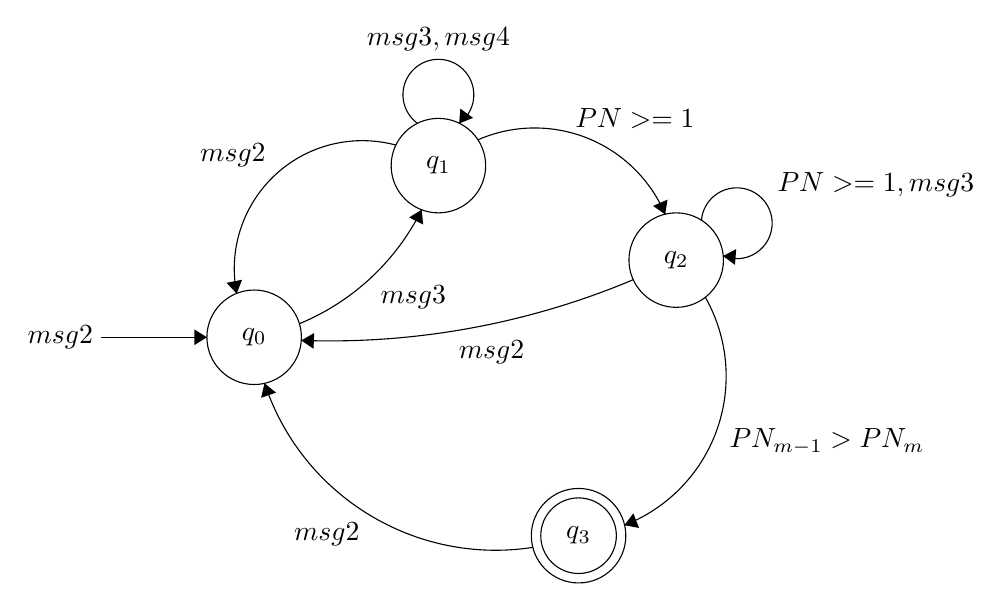
\begin{tikzpicture}[scale=0.2]
\tikzstyle{every node}+=[inner sep=0pt]
\draw [black] (22.6,-22.1) circle (3);
\draw (22.6,-22.1) node {$q_0$};
\draw [black] (34.3,-11.2) circle (3);
\draw (34.3,-11.2) node {$q_1$};
\draw [black] (49.4,-17.2) circle (3);
\draw (49.4,-17.2) node {$q_2$};
\draw [black] (43.2,-34.7) circle (3);
\draw (43.2,-34.7) node {$q_3$};
\draw [black] (43.2,-34.7) circle (2.4);
\draw [black] (12.9,-22.1) -- (19.6,-22.1);
\draw (12.4,-22.1) node [left] {$msg2$};
\fill [black] (19.6,-22.1) -- (18.8,-21.6) -- (18.8,-22.6);
\draw [black] (36.799,-9.565) arc (113.64657:23.01253:9.009);
\fill [black] (48.7,-14.3) -- (48.85,-13.36) -- (47.93,-13.76);
\draw (46.78,-8.89) node [above] {$PN>=1$};
\draw [black] (21.494,-19.33) arc (-168.7936:-285.26104:8.135);
\fill [black] (21.49,-19.33) -- (21.83,-18.45) -- (20.85,-18.64);
\draw (21.25,-11.31) node [above] {$msg2$};
\draw [black] (33.239,-14.001) arc (-26.43088:-67.62377:15.095);
\fill [black] (33.24,-14) -- (32.44,-14.49) -- (33.33,-14.94);
\draw (32.7,-18.81) node [below] {$msg3$};
\draw [black] (32.977,-8.52) arc (234:-54:2.25);
\draw (34.3,-3.95) node [above] {$msg3, msg4$};
\fill [black] (35.62,-8.52) -- (36.5,-8.17) -- (35.69,-7.58);
\draw [black] (51.001,-14.677) arc (175.32869:-112.67131:2.25);
\draw (55.8,-12.42) node [right] {$PN>=1, msg3$};
\fill [black] (52.38,-16.94) -- (53.13,-17.5) -- (53.21,-16.5);
\draw [black] (51.244,-19.552) arc (29.63405:-68.65106:10.156);
\fill [black] (46.11,-34.03) -- (47.04,-34.21) -- (46.68,-33.28);
\draw (52.75,-28.73) node [right] {$PN_{m-1}>PN_m$};
\draw [black] (46.671,-18.445) arc (-67.19541:-92.08203:49.722);
\fill [black] (25.59,-22.3) -- (26.37,-22.83) -- (26.41,-21.83);
\draw (37.67,-22.27) node [below] {$msg2$};
\draw [black] (40.298,-35.442) arc (-81.20921:-161.69491:15.457);
\fill [black] (23.26,-25.02) -- (23.04,-25.94) -- (23.99,-25.62);
\draw (27.21,-33.85) node [below] {$msg2$};
\end{tikzpicture}
\end{center}
\caption[State machine of the 4-way handshake with acceptance state of the KRACK attack]{State machine of the 4-way handshake with acceptance state of the KRACK attack.}
 \label{fig:stateMachineAttack}
\end{figure}

We receive many different types of frames but except the EAPOL frames and encrypted data frames, we ignore them. When we get in a specific state of the machine a different input than we expected (that is not listed next to transitions), we ignore it and stay in the same state. The initial state of the machine is the state $q_0$. We transition there when we receive \textit{message~2} and we store a value of the SNonce used in this message. When we get \textit{message~3}, we transition to the state $q_1$. We store the ANonce used in this message and now, we uniquely identified the handshake. We are waiting for encrypted data frames in $q_1$. When we get them, we are looking at the packet number received. It can and it will be reset after the handshake is finished, but we have to store the information about it to recognize when it happened for the second time. We look at two scenarios with one uniquely identified handshake. First, we detect the packet number is reset twice. Second, we missed the encrypted data frame with the reset packet number but we got another data frame and its packet number is lower than the one we have seen before. These two scenarios are listed in states $q_1$, $q_2$, $q_3$. In the acceptance state $q_3$, the KRACK attack is detected.




\chapter{Implementation}
\label{chap:implementation}

For our implementation, we chose to use programming language Python and package Scapy. It allows us to handle incoming and outcoming frames and also provides helpful tools for parsing the data. We ran it on Kali Linux and five Alfa AWUS036NHA Wi-Fi USB adapters. They have chipset Atheros AR9271, so we used driver ath9k\_htc for all of them. For running the attack, we used the same setup with two Alfa AWUS036NHA Wi-Fi USB adapters.

\section{Structure}
The structure of the detection tool consists of six files. We will explain what they are used for:

\begin{description}
\item \textbf{krackdetect.py} This file contains the main input function and class Detector which handles the detection process, meaning creating other classes, handling received messages and writing to possible \texttt{.pcap} file. There are two important functions \texttt{handle\_EAPOL}, which handles incoming EAPOL frames and \texttt{handle\_encrypted\_data}, which handles incoming encrypted data frame.
\item \textbf{NetworkMonitor.py} The file contains a class NetworkMonitor. The function methods handle the network-manager service, the interfaces and handle turning on and down the monitoring. It provides for example method like \texttt{configure\_interface\_for\_monitoring}, which sets the interface up and sets it to monitor mode. For this purpose, we use \texttt{ifconfig}, \texttt{iwconfig} and \texttt{airmon-ng} tools. Other methods are for example, set the channel to interface and turn on or off the network-manager to do not interfere with the monitoring.
\item \textbf{Util.py} The file contains functions for parsing data from frames as a sequence number, replay counter, packet number and a number of a message of the 4-way handshake. Also, there is a function which creates an identifier for a pair of a client and an AP based on their MAC addresses.
\item \textbf{Logger.py} Only handles log messages sent to the terminal. The messages have 6 levels of severity. In case of an attack it is a message of severity "ERROR".
\item \textbf{ListenSocket.py} Class initiating the L2Listen socket for monitoring, it also implements \texttt{recv} which returns 802.11 layer of the captured frame; \texttt{close} function closes the socket. We can use either this class or sniff function.
\item \textbf{PairState.py} The class represents a pair of an AP and a client performing the 4-way handshake. The function \texttt{handle\_msg} reacts to incoming messages and stores necessary data like nonces.  
\end{description}

\section{Encountered Problems}

We encountered several problems during the implementation of the detection tool. The attack itself is quite hard to be implemented. It is necessary to have an extensive background knowledge of the Wi-Fi standard and proper hardware and software. Additionally, we have to find vulnerable devices.
Also, some of the handshakes that are vulnerable are very hard to monitor and study because either their messages are always encrypted or only some devices support them. Thus, it is more complicated to trigger them. Besides, different devices behave a bit different, meaning, for example, some of them will not accept the retransmitted \textit{message~3} until they get a retransmitted \textit{message~1} first. And still, every device can monitor only on one channel. It means that for reliable monitoring of other attacking device we need four monitoring Wi-Fi cards, two for the attack itself and two for monitoring the attack from an outside perspective. 
After all, the detection itself is pretty straightforward. 

\section{Usage}
It is possible to use more interfaces and more channels. The first interface will be put to the first channel listed in the command, the second to the second one, etc. When it is not possible to set the listed interface to the monitor mode, it will throw an error, if none of the interfaces can be set to monitor mode, the process exits. To reduce interference between individual interfaces, try to keep them at least a meter in distance to each other.

\newpage
The system is run as a command-line tool and can be used as follows:

\begin{lstlisting}[language=bash, basicstyle=\tiny]
usage: krackdetect.py [-h] -i INTERFACE [INTERFACE ...] -ch CHANNEL
                      [CHANNEL ...] [-d DUMP] [-q [Q]]

Detection of Key Reinstallation Attacks (KRACKs)

optional arguments:
  -h, --help            show this help message and exit
  -i INTERFACE [INTERFACE ...], --interface INTERFACE [INTERFACE ...]
                        interfaces for monitoring the network
  -ch CHANNEL [CHANNEL ...], --channel CHANNEL [CHANNEL ...]
                        channel at which the traffic will be monitored
  -d DUMP, --dump DUMP  dumps captured data to .pcap file
  -q [Q]                quiet
  

\end{lstlisting}

\chapter{Testing and Evaluation}
\label{chap:testing}

This chapter deals with the testing part of the thesis. First, we tested a set of devices for vulnerability. Second, we tested our developed system for detection of the KRACK attacks against the 4-way handshake.

\section{Device Vulnerability}

We used the testing tool published by Vanhoef and introduced in Subsubsection~\ref{subsub:officialTestingScripts} to test a set of devices predominantly with iOS and Android operating systems. The test results are listed in Table~\ref{fig:tableTests}. We can see that according to the testing script, all of the devices are vulnerable to the GTK reinstallation during the 4-way or group key handshake. We found four Android devices vulnerable to the PTK reinstallation. One of them still reinstalls the all-zero key and so, allows the adversary to decrypt all data. Besides, we can see none of the iOS devices tested were vulnerable to the PTK reinstallation, even though, we also tested iOS version 9.3.5 which is not supported by the vendor anymore.

We also tested the vulnerability of the FT handshake on two the same AP devices UniFi~AP-AC-Pro (testing only one, without another device supporting 802.11r is not possible). And both were not vulnerable to the attack.  

\section{Attack Detection}

Due to the nature of the implementation, we have decided to test our detection system by measuring the percentage of correctly detected attacks and the percentage of reported false alarms. For both, we tested the system in environment defined in Section~\ref{enum:environments}, environment~\ref{env:B}.

\subsection{False Alarms}
To figure out if our detection system triggers alerts as false positives, we assumed the tested environment is secure when we are not performing the attack. We set up two Wi-Fi APs on channels 1 and 9 in the environment. To run our script, we used five external Wi-Fi cards and set them to channels 1, 3, 5, 7, and 9 respectively. We let it run for three hours in the defined environment during the day during the standard operation. And we watched detected attacks. We did not detect any false alarms so, we consider our script in this term reliable.

\subsection{Detected Attacks}
We used two Wi-Fi NICs for the attack and three for the detection. We assumed we do not know which channel will the attacker use to clone the real AP to. However, we know which channels are our Wi-Fi APs running on. Thus, we used the channels 1 and 9 and the third we decided by random choice to set to 5. We made a few different scenarios in terms of the relative position of the detection tool, the attacker, attacked client and the real AP.  
In all these scenarios, we were still inside the flat described in Section~\ref{enum:environments}, environment~\ref{env:B}, thus, we had a decent signal for monitoring of at least one of the three participants in the attack (the AP, the client, the attacker). The detection tool was able to detect all successful attacks in all scenarios. Thus, we can say that in an average environment in terms of interference and device distances, we are able to detect the attack reliably. Also, it is enough to be able to monitor either the side of the AP or the side of the client, in channel based MitM, to be able to detect the KRACK attacks. 

\section{Comparison to Other Tools}

During the research, we found only one other tool for dealing with the same problem. It is available in~\cite{securingsam_2017}. This tool runs on the AP in a network and detects only retransmission of the \textit{message~3} of the handshake. This retransmission can happen even if there is no attack and the script does not have any chance to verify that the attack was performed or in case it was that it was successful. Optionally, in case it detects this retransmission, it disassociates and deauthenticates the client from the AP. This approach can lead to a lot of false positives and worsen the service provided by the AP. It runs only on APs with Python available.

\section{Evaluation}
There were many mobile devices tested for their vulnerability to the KRACK attacks. Even though, it has been more than a year since the publication of the vulnerability, some of them are still not patched. 

According to testing of our detection system, in case we are in a decent range for monitoring the attacked client or the AP, in a place with no significant interference, we reliably detect the attack.

\begin{center}
\begin{table}[h!]
\begin{tabular}{|c|c|c|c|}
\hline
\textbf{Device} & \textbf{OS} & \textbf{PTK reinstall} & \textbf{GTK reinstall}  \\ \hline \hline
Asus~Z007 & Android~4.4.2 & vulnerable &  vulnerable \\ \hline
Samsung~SM-G530H & Android~4.4.4 & vulnerable & vulnerable \\ \hline
Asus~Nexus~7 & Android~5.1.1 & vulnerable & vulnerable \\ \hline
myPhone~Pocket  & Android~6.0 & not vulnerable & vulnerable \\ \hline
LGE~Nexus 5 & Android~6.0.1 & all-zero key & vulnerable \\ \hline
OPPO~R9s~Plus & Android~6.0.1 & not vulnerable & vulnerable \\ \hline
AllView~P41~eMagic  & Android~7.0 & not vulnerable & vulnerable  \\ \hline
Huawei~VNS-L21 & Android~7.0 & not vulnerable & vulnerable \\ \hline
Xiaomi~Redmi~Note~4 & Android~7.0 & not vulnerable & vulnerable \\ \hline
Huawei~Ane-LX1 & Android~8.0 & not vulnerable & vulnerable \\ \hline
Huawei~ATU-L31 & Android~8.0 & not vulnerable & vulnerable \\ \hline
Huawei~MHA.AL00 & Android~8.0 & not vulnerable &
 vulnerable \\ \hline
Samsung~SM-A320FL & Android~8.0 & not vulnerable & vulnerable  \\ \hline
Samsung~SM-G950F & Android~8.0 & not vulnerable & vulnerable \\ \hline
Samsung~SM-J330F  & Android~8.0 & not vulnerable & vulnerable  \\ \hline
LGE~Nexus~5X & Android~8.1.0 & not vulnerable & vulnerable \\ \hline
Xiaomi~Mi~A2~Lite & Android~8.1.0 & not vulnerable & vulnerable  \\ \hline
iPad mini & iOS~9.3.5 & not vulnerable & vulnerable \\ \hline
iPhone 6 & iOS~11.4 & not vulnerable & vulnerable  \\ \hline
iPhone 6 Plus & iOS~11.4.1 & not vulnerable & vulnerable   \\ \hline
iPhone 7 & iOS~12.1.1 & not vulnerable & vulnerable \\ \hline
iPhone X & iOS~12.1.2 & not vulnerable & vulnerable \\ \hline
\end{tabular}
\caption[Results of device vulnerability testing]{Results of device vulnerability testing.}
\label{fig:tableTests}
\end{table}
\end{center}

\setsecnumdepth{part}

\chapter{Conclusion}
\label{chap:conclusion}

This thesis aimed to study the KRACK attacks and analyze its traffic. It also proposes a tool for testing device vulnerability and creates a system for KRACK detection in real-time. 

The KRACK attacks exploit a vulnerability found in the standard 802.11i defining WPA2 protocol. It is the only Wi-Fi data security protocol that was considered secure for more than a decade. Most of us use Wi-Fi every day and often do not think about data we send over it. Thus, when Mathy Vanhoef found this vulnerability and published it in October 2017, it became a media stunt. The vast majority of Wi-Fi devices were affected by this vulnerability. Also, it meant that all data we send over Wi-Fi might be possibly decrypted. 

In this work, we studied the principle of the KRACK attacks vulnerability. For this purpose, it was necessary to become acquainted with parts of the Wi-Fi standard and with research behind it. Based on what we studied, the thesis describes the process of Wi-Fi client connection, and the principle of the KRACK attacks vulnerability, its practical impact, and countermeasures. We found that the implementation of the attack is quite complicated, but we modified the proof-of-concept scripts and managed to perform the attack against a few vulnerable mobile devices. Thus, we were able to monitor both standard, and malicious traffic of the 4-way handshake and data frames sent after it. We have created a lab consisting of five Wi-Fi NICs that were switched into monitor mode, and tools to capture and transmit Wi-Fi frames. The lab was used for practical experiments described in this thesis. Based on what we studied and analyzed, we made a list of characteristics that make the attack detectable. The results are also contained in this thesis.

We have proposed the tool for testing device vulnerability and used an existing solution for testing more than twenty mobile devices. We found some of them vulnerable and also, we found a device that still reinstalls the all-zero-key. Besides, we proposed a system for detection of the KRACK attack in real-time. The developed scripts detect the attack against the 4-way handshake by detecting retransmission of the third message of the 4-way handshake and following reinstallation of the session key. In a typical environment with not extremely high interference, the script works reliably and does not trigger any false alarms.

Even though the thesis has met the set goals, the extension of the detection system might be a beneficial future work. Also, the analysis of other handshakes from the standard for vulnerabilities could help improve Wi-Fi security. The topic is extensive, and I found this work a decent basis for future extension.



\bibliographystyle{iso690}
\bibliography{ref}

\setsecnumdepth{all}
\appendix
\printglossaries
\chapter{802.11 Significant Family Standards and Amendments}
\label{app:802.11}

\begin{description}
\item [802.11 (1997)] The initial standard which provided 1 or 2 Mbps transmission in the 2.4 GHz band using either \gls{fhss} or \gls{dsss}. %\cite{ieee802.11_1997}. 

\item [802.11a (1999)] It operates at the 5 GHz ISM\Anote{id1} band with the theoretical data rates up to 54 Mbps. The modulation techique used is OFDM. % \cite{HI10}.

\item [802.11b (1999)] IEEE 802.11b was the first wireless LAN standard to be widely adopted and built in to many laptop computers and other forms of equipment \cite{PHY13}. It operates at the 2.4 GHz ISM band with theoretical data rates up to 11 Mbps. Although the IEEE 802.11a standard was introduced at the same time and was capable of higher speeds, it did not catch on in the same way. The main reason for this was that it operated in the 5 GHz ISM band rather than the 2.4 GHz of 802.11b, and this made it more expensive \cite{PHY13}. %\cite{PHY13}. 

\item [802.11d (2001)] International (country-to-country) roaming extensions

\item [802.11e (2005)] Quality of Service (QoS) and prioritization

\item [802.11g (2003)] Like 802.11b, its predecessor, 802.11g operates in the 2.4 GHz ISM band. It provides a maximum raw data throughput of 54 Mbps. Although the system is compatible with 802.11b, the presence of an 802.11b participant in a network significantly reduces the speed of a net. In fact, it was compatibility issues that took up much of the working time of the IEEE 802.11g committee. The main modulation method chosen for 802.11g was that of OFDM. It soon took over from the b standard and it became the dominant Wi-Fi technology \cite{RE18}. 

\item [802.11h (2003)] Power control

\item [802.11i (2004)] Document deals with authentication and encryption. Its partial implementation is called WPA and full is called WPA2. It defines the 4-way handshake, the PeerKey handshake and the group Key handshake \cite{ieee802.11i_2004}, all vulnerable to the KRACK attacks \cite{VA17}. These handshakes are further discussed in the section \ref{sec:security}.

\item [802.11k (2008)] Measurement reporting

\item [802.11r (2008)] It is also called Fast BSS Transition (or fast roaming). It describes technology to permit continuous connectivity aboard wireless devices in motion. The Fast BSS Transition handshake is also vulnerable to the KRACK attacks and so \cite{VA17}, it will be also explained further in the section \ref{sec:security}. This standard also slightly extends the 4-way handshake and provides a detailed state machine of the supplicant \cite{ieee802.11r_2008}.

\item[802.11n (2009)] It uses multiple antennas to increase data rates. As the first Wi-Fi standard that introduced MIMO (Multiple-Input and Multiple-Output) support. The purpose of the standard is to improve network throughput over the two previous standards—802.11a and 802.11g—with a significant increase in the maximum net data rate from 54 Mbit/s to 600 Mbit/s with the use of four spatial streams at a channel width of 40 MHz. It can be used in the 2.4 GHz or 5 GHz frequency bands. The devices supporting this technology are certified as Wi-Fi 4 by the WFA \cite{wi-fi6}.

\item[802.11p (2010)] Wireless Access for the Vehicular Environment

\item[802.11s (2011)] Mesh networking

\item[802.11u (2011)] It adds features that improve interworking with networks like 3G / cellular and other forms of external networks.

\item[802.11v (2011)] Deals with \gls{wnm} and device configuration. This amendment defines a WNM-Sleep mode. In \cite{VA_ccs2018}, author of the KRACK attack describes a way how to abuse WNM-Sleep response frames to trigger key reinstallation. 

\item[802.11w (2009)] Protected Management Frames security enhancement

\item[802.11y (2008)] Contention Based Protocol for interference avoidance

\item[802.11z (2010)] Defines mechanism called \gls{tdls} enabling user to directly transfer data between two Wi-Fi clients that are part of the same Wi-Fi network. The TDLS PeerKey handshake is defined for this purpose and is also vulnerable to the KRACK attacks \cite{VA_ccs2018} and will be further discussed in the section \ref{sec:security}.

\item[802.11aa (2012)] Enhancements to 802.11 MAC for robust audio streaming while maintaining coexistence with other types of traffic.

\item[802.11ac (2013)] Standard providing high-throughput WLANs on the 5 GHz band. The specification has multi-station throughput of at least 1 gigabit per second and single-link throughput of at least 500 megabits per second (500 Mbit/s). This is accomplished by extending the air-interface concepts embraced by 802.11n: wider RF bandwidth (up to 160 MHz), more MIMO spatial streams (up to eight), downlink multi-user MIMO (up to four clients), and high-density modulation (up to 256-QAM). The devices supporting this technology are certified as Wi-Fi 5 by the WFA. This standard also extends GCMP data-confidentiality protocol by adding support for 256-bit keys.

\item[802.11ad (2012)] It was developed to provide a \gls{mgws} standard at 60 GHz frequency.
Nowadays, it is rolled out under trademark \gls{wigig}. It has limited range (just a few meters and difficult to pass through physical obstacles) compares to other conventional Wi-Fi systems. However, the high frequency allow it to utilize more bandwidth which in turn enable the transmission of data at high data rate up to multiple gigabit per second. This standard also defines a new data-confidentiality protocol for data encryption called \gls{gcmp}.

\item[802.11af (2013)] Wi-Fi in TV spectrum white spaces (often called White-Fi). 

\item[802.11ai (2016)] The document provides \gls{fils} methods to enhance end user experience in dense environments. This function enables a wireless LAN client to achieve a secure link setup within 100ms. The FILS handshake is also vulnerable to the KRACK attack \cite{VA_ccs2018} and will be further discussed in the section \ref{sec:security}. %\cite{ieee-sa_ai}

\item[802.11ax (under development)] New standard under development which release is planned on to 2019. The devices supporting this technology will be certified as Wi-Fi 6 by the WFA.
\end{description}
\include{C_cveIdentifiers}
\chapter{802.11 Frames Subtypes}
\label{app:frameSubtypes}

\begin{center}
\begin{longtable}{|c|c|c|}
\hline
\textbf{Type Value} & \textbf{Subtype Value} & \textbf{Subtype Description}   \\ \hline \hline
00 & 0000 & Association Request  \\  \hline
00 & 0001 & Association Response   \\  \hline
00 & 0010 & Reassociation Request   \\  \hline
00 & 0011 & Reassociation Response    \\  \hline
00 & 0100 & Probe Request    \\  \hline
00 & 0101 & Probe Response     \\  \hline
00 & 0110-0111 & Reserved  \\  \hline
00 & 1000 & Beacon \\  \hline
00 & 1001 & ATIM    \\  \hline
00 & 1010 & Disassociation     \\  \hline
00 & 1011 & Authentication     \\  \hline
00 & 1100 & Deauthentication     \\  \hline
00 & 1101 & Action     \\ \hline
00 & 1110-1111 & Reserved     \\  \hline
01 & 0000-0111 & Reserved    \\  \hline
01 & 1000 & Block Ack Request    \\  \hline
01 &1001 & Block Ack    \\  \hline
01 &1010 & PS-Poll    \\  \hline
01 &1011 & RTS     \\  \hline
01 &1100 & CTS     \\  \hline
01 &1101 & ACK     \\  \hline
01 &1110 & CF-end     \\  \hline
01 &1111 & CF-end + CF-ack    \\  \hline
10 & 0000 & Data   \\  \hline
10 & 0001 & Data + CF-ack    \\  \hline
10 & 0010 & Data + CF-poll    \\  \hline
10 & 0011 & Data +CF-ack +CF-poll     \\  \hline
10 & 0100 & Null    \\  \hline
10 & 0101 & CF-ack     \\  \hline
10 & 0110 & CF-poll    \\  \hline
10 & 0111 & CF-ack +CF-poll     \\  \hline
10 & 1000 & QoS data    \\  \hline
10 & 1001 & QoS data + CF-ack    \\  \hline
10 &1010 & QoS data + CF-poll    \\  \hline
10 &1011 & QoS data + CF-ack + CF-poll    \\  \hline
10 &1100 & QoS Null    \\ \hline
10 &1101 & Reserved  \\  \hline
10 &1110 & QoS + CF-poll (no data)    \\ \hline
10 &1111 & Qos + CF-ack (no data)   \\ \hline
10 &0000 & Reserved    \\  \hline

\caption[802.11 frame subtypes]{Subtypes of 802.11 management, control and data frames}
\label{tab:frames_subtypes}
\end{longtable}
\end{center}

\chapter{Contents of enclosed CD}

%change appropriately

\begin{figure}
	\dirtree{%
		.1 readme.txt\DTcomment{the file with CD contents description}.
		.1 src\DTcomment{the directory of source codes}.
		.2 krackdetect\DTcomment{implementation sources}.
		.2 thesis\DTcomment{the directory of \LaTeX{} source codes of the thesis}.
		.2 traffic\DTcomment{example of captured traffic}.
		.1 text\DTcomment{the thesis text directory}.
		.2 thesis.pdf\DTcomment{the thesis text in PDF format}.
	}
\end{figure}
\end{document}
